\documentclass[a4paper,11pt,final]{article}
\usepackage[margin=1.5cm]{geometry}

\usepackage[english,./french]{babel}
\usepackage[utf8]{inputenc}
\usepackage[T1]{fontenc}
\usepackage[pdftex]{graphicx}
\usepackage{setspace}
\usepackage{hyperref}
\usepackage[french]{varioref}
\usepackage{siunitx}

\newcommand{\reporttitle}{Etats de diffusion pour l’équation de Schrödinger 1D stationnaire}     % Titre
\newcommand{\reportauthor}{Jean \textsc{Dupont}\\ Louis \textsc{Martin}} % Auteur
\newcommand{\reportsubject}{Projet informatique} % Sujet
\newcommand{\HRule}{\rule{\linewidth}{0.5mm}}
\setlength{\parskip}{1ex} % Espace entre les paragraphes

\hypersetup{
    pdftitle={\reporttitle},%
    pdfauthor={\reportauthor},%
    pdfsubject={\reportsubject},%
    pdfkeywords={rapport} {vos} {mots} {clés}
}

\begin{document}
  % Inspiré de http://en.wikibooks.org/wiki/LaTeX/Title_Creation

\begin{titlepage}

\begin{center}


\includegraphics [width=190mm]{logo-PHYSIQUE.jpg} 
\textsc{ }\\
\textsc{ }\\
\textsc{\LARGE Université Claude Bernard Lyon 1}\\
\textsc{ }\\
\textsc{ }\\
\textsc{\LARGE Master Physique}\\
\textsc{ }\\
\textsc{ }\\

\textsc{\Large \reportsubject}\\[0.5cm]
\HRule \\[0.4cm]
{\huge \bfseries Etats de diffusion pour l’équation de Schrödinger 1D stationnaire}\\[0.4cm]
\HRule \\[1.5cm]

\begin{minipage}[t]{0.3\textwidth}
  \begin{flushleft} \large
    \emph{Auteurs :}\\
    \textsc{Le Carrer Correntin} 
    \newline \textsc{Selahiye Aras}
  \end{flushleft}
\end{minipage}
\begin{minipage}[t]{0.6\textwidth}
  \begin{flushright} \large
    \emph{Encadrant :} \\
     \textsc{Abdul Rahman ALLOUCHE} 
  \end{flushright}
\end{minipage}


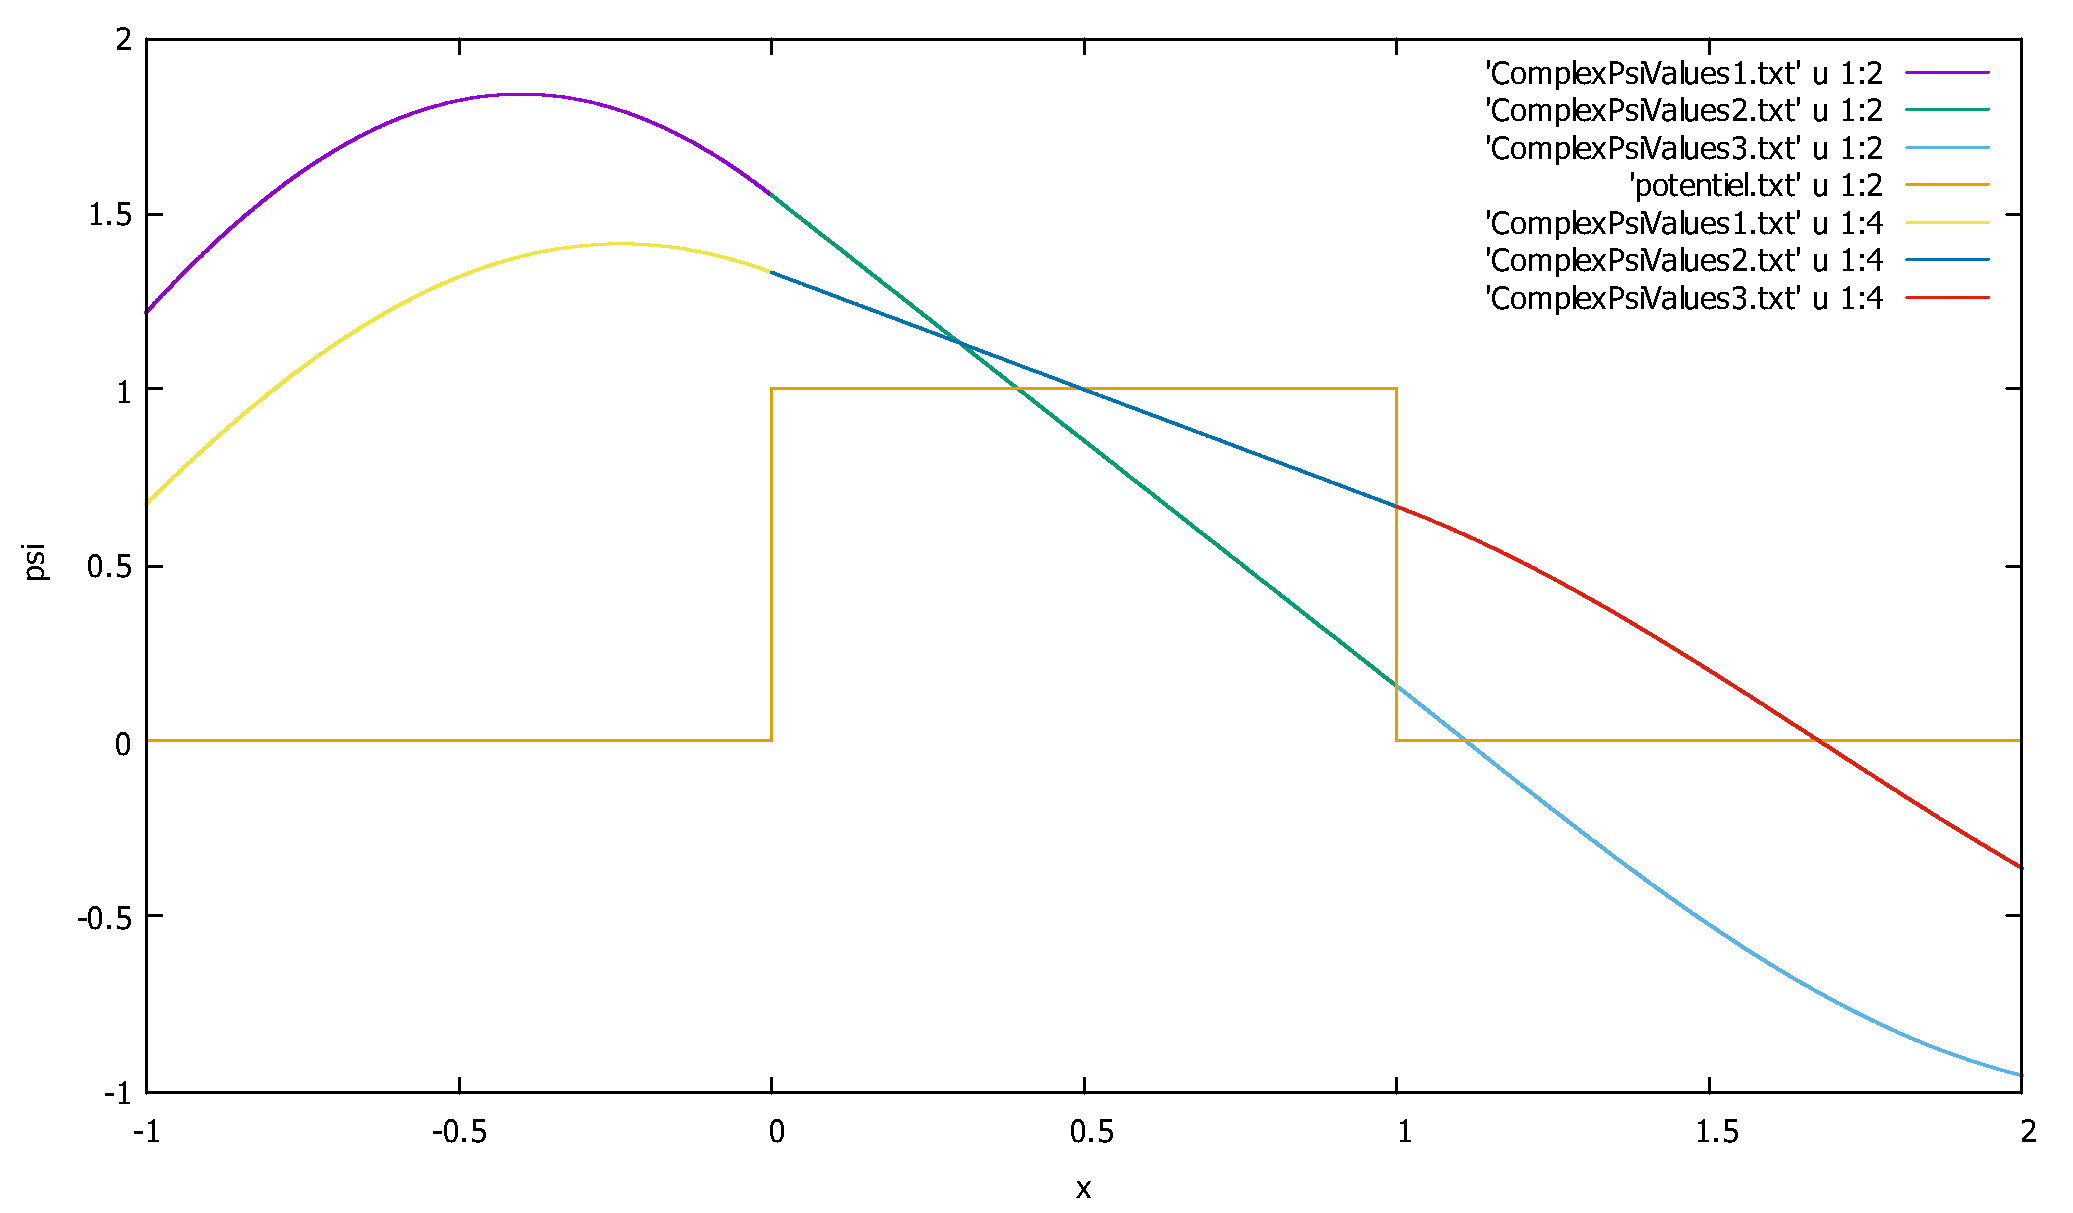
\includegraphics[width=150mm]{potentiel 1 barrier/Reel(psi(x))_2methods.pdf}
\vfill
   
{\large 18 avril 2023}

\end{center}

\end{titlepage}

  \cleardoublepage 
  \tableofcontents % Table des matières
  \sloppy          % Justification moins stricte : des mots ne dépasseront pas des paragraphes
  \cleardoublepage
  
  \section*{Introduction}
\addcontentsline{toc}{section}{Introduction}

\par Notre projet porte sur la résolution de l’équation  de Schrödinger stationnaire à une dimension, afin de déterminer les coefficients de réflexion et de transmission d’une particule à travers  un potentiel. Notre programme va résoudre l’équation de Schrödinger numériquement par deux méthodes. Pour vérifier la validité de la résolution numérique notre programme comparera le résultat à la valeur analytique connue pour une barrière de potentiel simple. Dans un premier temps nous reviendrons sur l’équation de Schrödinger, son principe et son utilisation, et nous présenterons les deux méthodes de résolution. Ensuite nous présenterons des résultats pour différents potentiels dont on ne connaît pas la solution analytique. Pour finir nous présenterons des résultats de la variation des différents paramètres, comme la masse du particule, la largeur du potentiel, pour une barrière de potentiel.


  \cleardoublepage
  \section{Principe physique et méthodes de résolution}

\subsection{Equation de schrodinger}
L’équation de Schrödinger tire son nom du physicien Erwin Schrödinger qui a créé cette équation en 1925 pour laquelle il a obtenu le prix Nobel de physique en 1933. L’équation de Schrödinger est une équation d’onde qui tient compte à la fois de l’énergie non relativiste et la quantification de celle-ci. L’équation de Schrödinger est une équation fondamentale de la physique quantique, elle décrit l’évolution dans l’espace et le temps d’une particule massive non relativiste. Pour notre projet nous nous intéresserons à l’équation de Schrödinger stationnaire\cite{texier2015mecanique}, c’est-à-dire que l’équation sera indépendante du temps. Nous nous intéresserons qu’a une seule dimension l’équation dépendra donc que d’une seul direction ici x.

\begin{equation} \label{eq:schrodinger}
 \frac{-\hbar^2}{2m}\frac{d^2\psi(x)}{dx^2 }+V(x)\psi(x)=E\psi(x)
\end{equation}
\begin{center}
$ V(x) = \left\{
    \begin{array}{ll}
       f(x) & \mbox{si}\ 0<x<a \\
       0 & \mbox{sinon.}
    \end{array}
\right.$
\end{center}

\subsection{Unité système atomique}

Pour résoudre l’équation de Schrödinger nous allons nous placer dans le système d'unités atomiques \cite{frwiki:193318984}et non pas dans le système internationale l'équivalence entre les deux système est donné dans le tableau \ref{tab1}. Le système d’unités atomiques est mieux adapté car nous travaillons sur de la physique quantique. Les unités atomiques sont défini en posant la constantes de planck réduite $\hbar$, la masse de l’électron $m_{e}$  et la constante de l'électrostatique $\frac{e^2}{4\pi\epsilon_{0}}$égale à 1.


\begin{table}[!ht]
\centering
\begin{tabular}{|l|l|l|l|}
\hline Grandeur & Nom &  Valeur SI  \\
\hline  Masse & masse de l'électron & 9,109 382 6× $10^{-31}$ kg  \\
\hline Longueur & rayon de Bohr & 5,291 772 109 2× $10^{-11}$ m\\ 
\hline Énergie & hartree & 4,359 744 17 × $10^{-18} $J \\
\hline
\end{tabular}
\caption{Equivalence SI et unité atomique}
\label{tab1}
\end{table}


\subsection{Méthodes de résolution utilisées}
En dehors du potentiel l'équation \ref{eq:schrodinger} devient :

\begin{equation} \label{eq:schrodinger2}
\frac{d^2\psi(x)}{dx^2 }=\frac{-2mE}{\hbar^{2}}\psi(x)
\end{equation}

\begin{equation} \label{eq:schrodinger3}
\frac{d^2\psi(x)}{dx^2 }=-k^{2}\psi(x)
\end{equation}

\begin{center}
$k=\sqrt{\frac{2mE}{\hbar^{2}}}$
\end{center}

La solution générale de l'équation de Schrödinger est $\psi(x)=Ae^{ikx}+Be^{-ikx}$.

L'équation de Schrödinger admettra différentes solutions selon la région du potentiel dans laquelle elle se trouve. Pour $x<0$ l'équation sera de la forme de la solution générale, dans la région $II$ on cherchera la solution numériquement. Enfin pour $x>a$ la propagation dans le sens des x négatif est impossible donc la fonction d'onde sera de la forme  $\psi(x)=Ce^{ikx}$.
\newpage 
\begin{center}
$\psi_{I}(x)=Ae^{ikx}+Be^{-ikx}\\$
$\psi_{II}(x)=clacule \ numérique\\$
$\psi_{III}(x)=Ce^{ikx}\\$
\end{center}


Notre objectif est de trouver les coefficients de réflexion et de transmission, c'est à dire la probabilité pour qu'une particule passe à travers le potentiel :

\begin{equation} \label{eq:defcoeff}
R=|\frac{B}{A}|^{2}\qquad T=|\frac{C}{A}|^{2}\qquad R+T=1
\end{equation}
\subsubsection{Méthode 1}

Pour la méthode 1 on fixe la constante C=1. On impose également la continuité des dérivées de la fonction d'onde en 0 et en a.
\begin{center}
$\psi'_{I}(0)=\psi'_{II}(0)$\\
$\psi'_{II}(a)=\psi'_{III}(a)$
\end{center}
En reprenant l'équation de Schrödinger du début \ref{eq:schrodinger} et en utilisent la formule de la dérivée seconde discrète\,\footnote{$\frac{d^{2}f(x)}{dx^{2}}=\frac{f(x+h)+f(x-h)-2f(x)}{h^{2}}$}. On obtient une équation \ref{eq:numregion2} qui permet de calculer successivement toutes les valeurs de la fonction d'onde dans la région $II$ afin d'obtenir la valeur de $\psi(0)$ et  la valeur de $\psi(pas)$. En utilisant la formule de la dérivée discrète\,\footnote{$\frac{df(x)}{dx}=\frac{f(x+h)+f(x-h)}{h}$} et les valeurs de $\psi$ on trouve la dérivée de la fonction d'onde en 0 ($\psi'_{II}(0)$).

\begin{equation} \label{eq:numregion2}
\psi(x-pas)=-\psi(x+pas)+(\frac{2mpas^{2}}{\hbar^{2}}(V(x)-E)+2)\psi(x)
\end{equation}

Avec la continuité des dérivées on obtient le système d'équation suivant qui permet de déterminer les valeurs des constantes A et B, et ainsi de déterminer les deux coefficients recherchés.
\begin{center}
$ \left\{
    \begin{array}{ll}
       A+B= \psi_{II}(0) \\
       ikA+ikB=\psi'_{II}(0) 
    \end{array}
\right.$
\end{center}
\subsubsection{Méthode 2}
Pour la méthode 2 on fixe la constante A=1.Puis on choisie une valeur de B aléatoire ($B_{i}$) puis on utilise l'équation  \ref{eq:numregion2} pour calculer successivement les valeurs de la fonction d'onde dans la région $II$ afin d'obtenir la valeur de$\psi_{II}(a)$. On trouve alors une valeur de C, on utilise de nouveau l'équation de résolution numérique de la fonction d'onde pour trouver la valeur de $\psi_{II}(0)$. On trouve donc une nouvelle valeur de B ($B_{f}$), on cherche à se que la valeur de $B_{i}$soit identique à la valeur de $B_{f}$ pour cela on utilise un algorithme de minimisation dans notre cas l'algorithme de descente de gradient. La minimisation permet donc de déterminer les valeurs de B et de C, et ainsi les coefficients de transmission et de réflexion.

\subsubsection{Vérification fonctionnement}

Afin de vérifier que le calcule des coefficients de transmission et de réflexion sont correct on utilise la solution analytique connue \cite{antoine2022introduction}{}de la barrière de potentiel simple. 
\newpage 
$E<V_{0}$
\qquad
$\alpha=\sqrt{\frac{2m}{\hbar}(V_{0}-E}$
\begin{equation} \label{eq:analityquee<v}
T=\frac{1}{1+\frac{V_{0}^{2}sinh^{2}(\alpha a)}{4E(V_{0}-E)}}
\end{equation}

$E=V_{0}$
\begin{equation} \label{eq:analityquee=v}
T=\frac{1}{1+\frac{V_{0}a^{2}\hbar^{2}}{2}}
\end{equation}

$E>V_{0}$
\qquad
$k=\sqrt{\frac{2mV_{0}a^{2}}{\hbar}(1-\frac{E}{V_{0}}}$
\begin{equation} \label{eq:analityquee>v}
T=\frac{1}{1+\frac{V_{0}^{2}sin^{2}(k)}{4E(E-V_{0})}}
\end{equation}
\\

\begin{table}[!ht]
\centering
Paramètres utilisés $E=1.2$,\ $a=1$,\ $m=1$,\ $V_{0}=1$,\ $N=20000$\\
\begin{tabular}{|l|l|l|}
\hline   & Méthode 2 & Analytique  \\
\hline  Méthode 1 &   1.0917944672395e-05 & 2.70045e-05 \\
\hline Méthode 2 &   &1.60866e-05\\ 
\hline
\end{tabular}
\caption{Écarts entre les méthodes et solution analytique}
\label{tab2}
\end{table}
  \cleardoublepage
  \section{Coefficients de réflexion et de transmission pour différent potentiel}

Avant de présenter les résultats des coefficients de réflexions et de transmissions pour les différents potentiels,pour lesquels on n'affichera la fonction d'onde que d'une méthode et que d'une seule partie du nombre complexe qui compose celle-ci.


\begin{figure}[!ht]
    \begin{minipage}[c]{.46\linewidth}
        \centering
        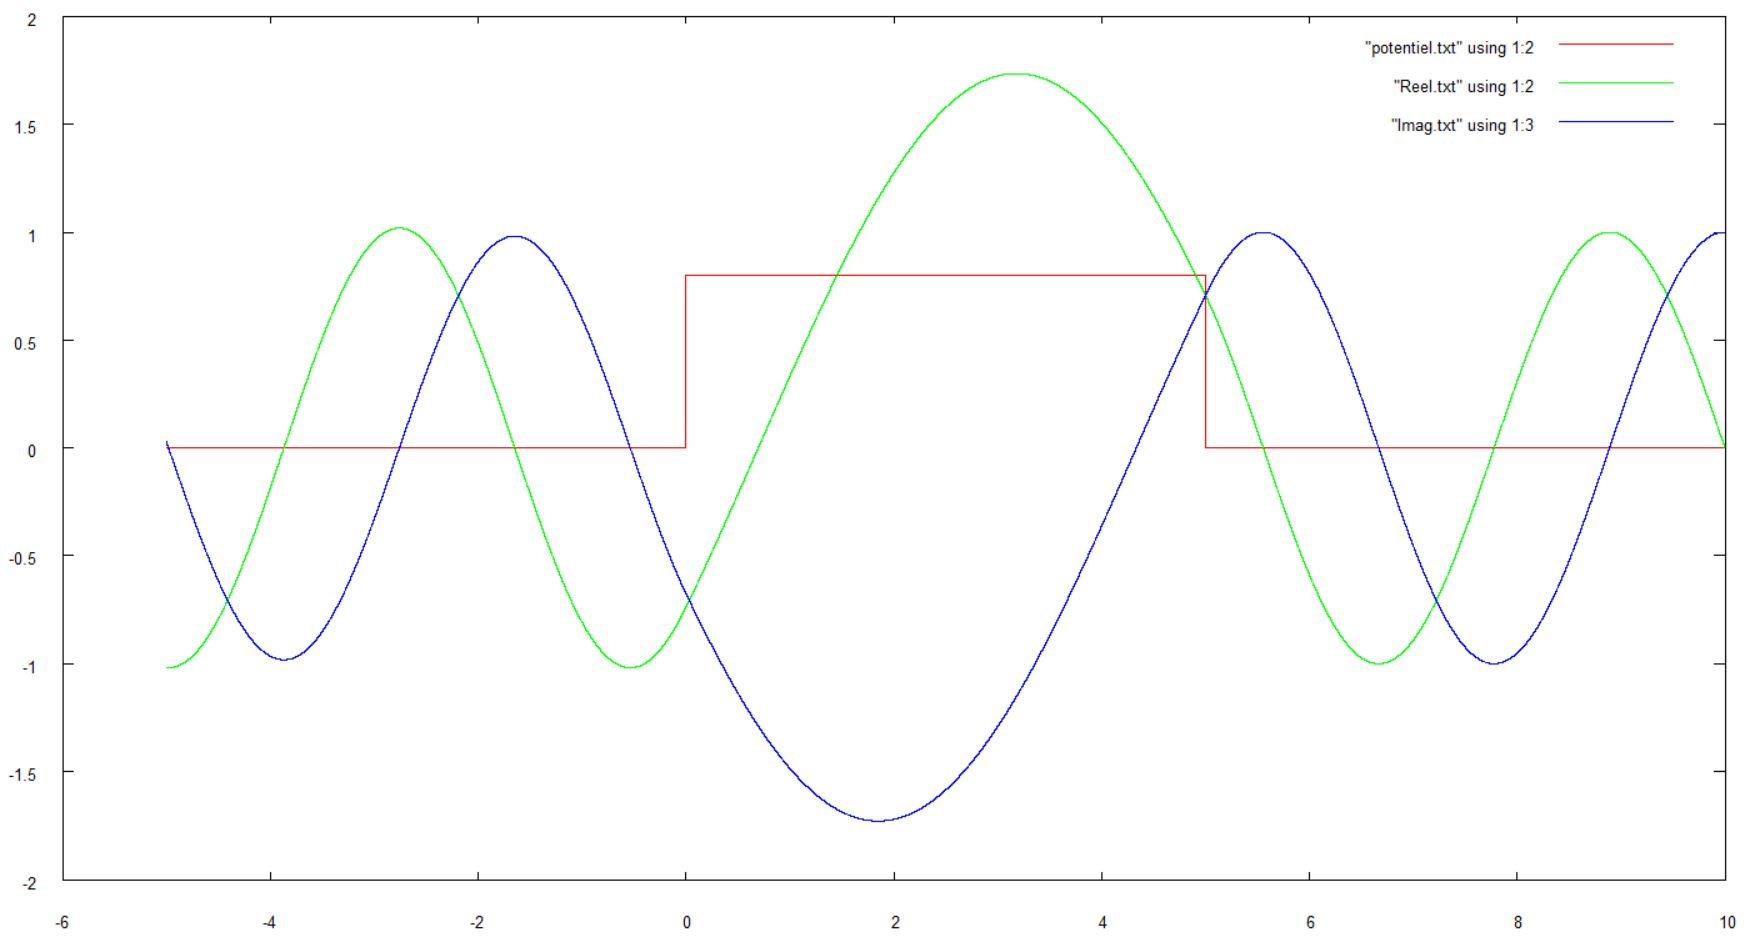
\includegraphics[width=0.9\textwidth]{imag et reel.jpg}
        \caption{Fonction d'onde réel et imaginaire}
    \end{minipage}
    \hfill%
    \begin{minipage}[c]{.46\linewidth}
        \centering
        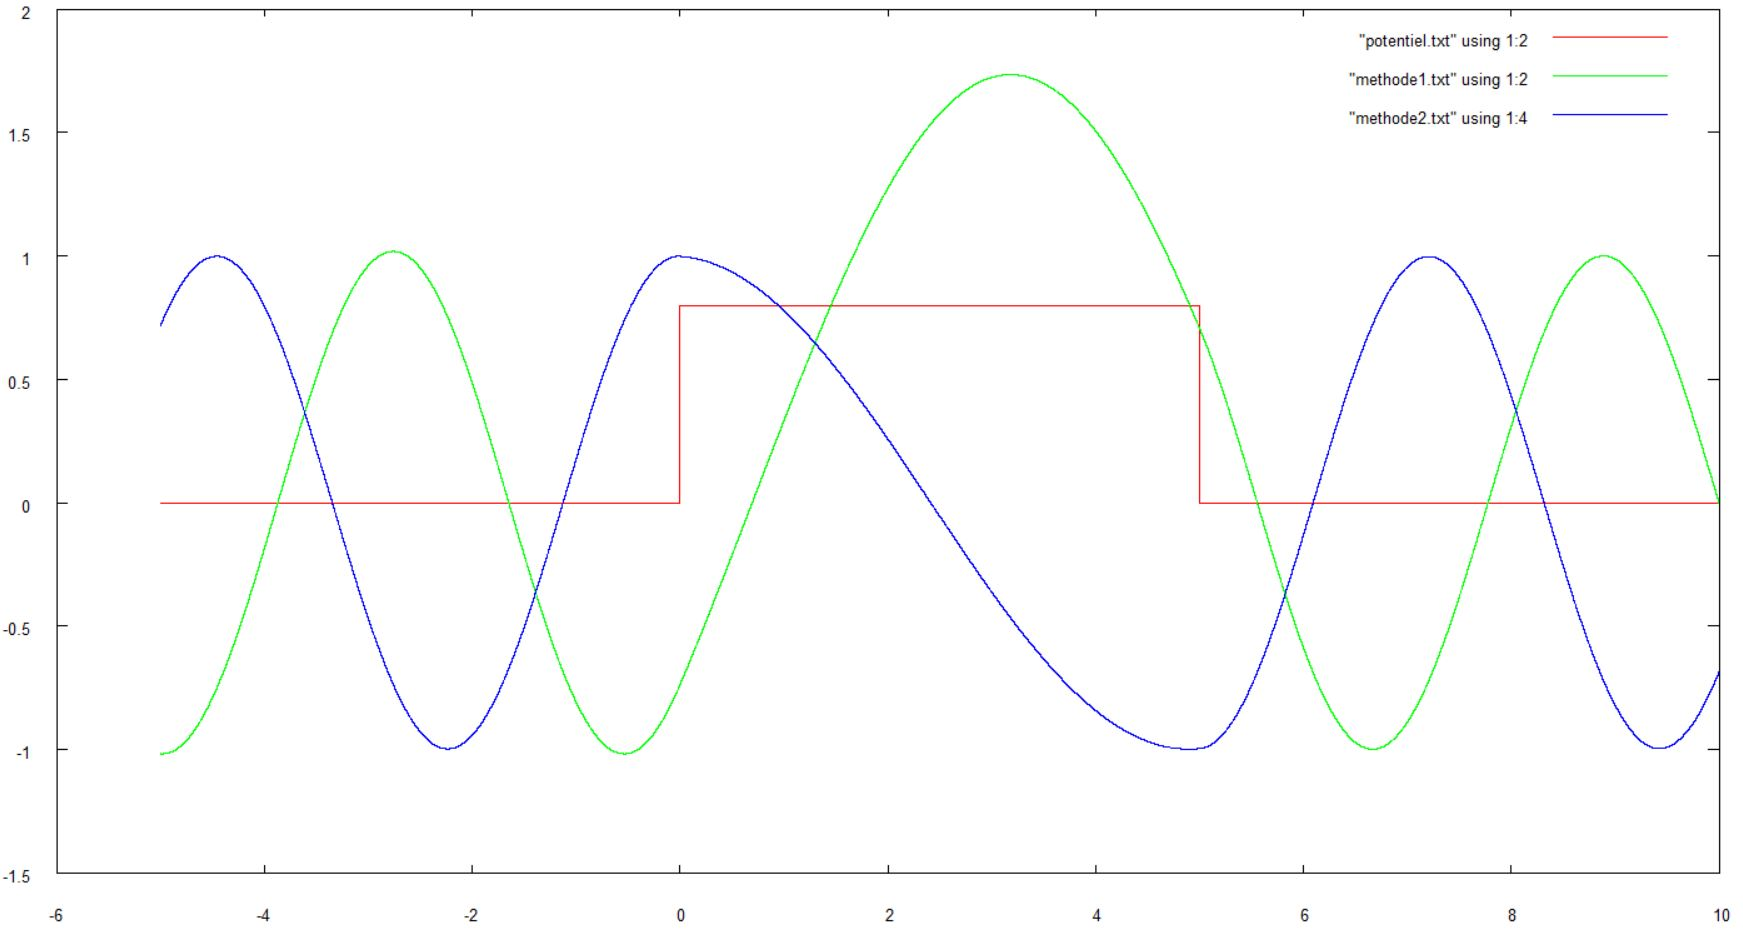
\includegraphics[width=0.9\textwidth]{methode12.jpg}
        \caption{Fonction d'onde réel méthode 1 et 2}
    \end{minipage}
\end{figure}

\subsection{Barrière de potentiel simple}

\begin{figure}[!ht]
    \center
    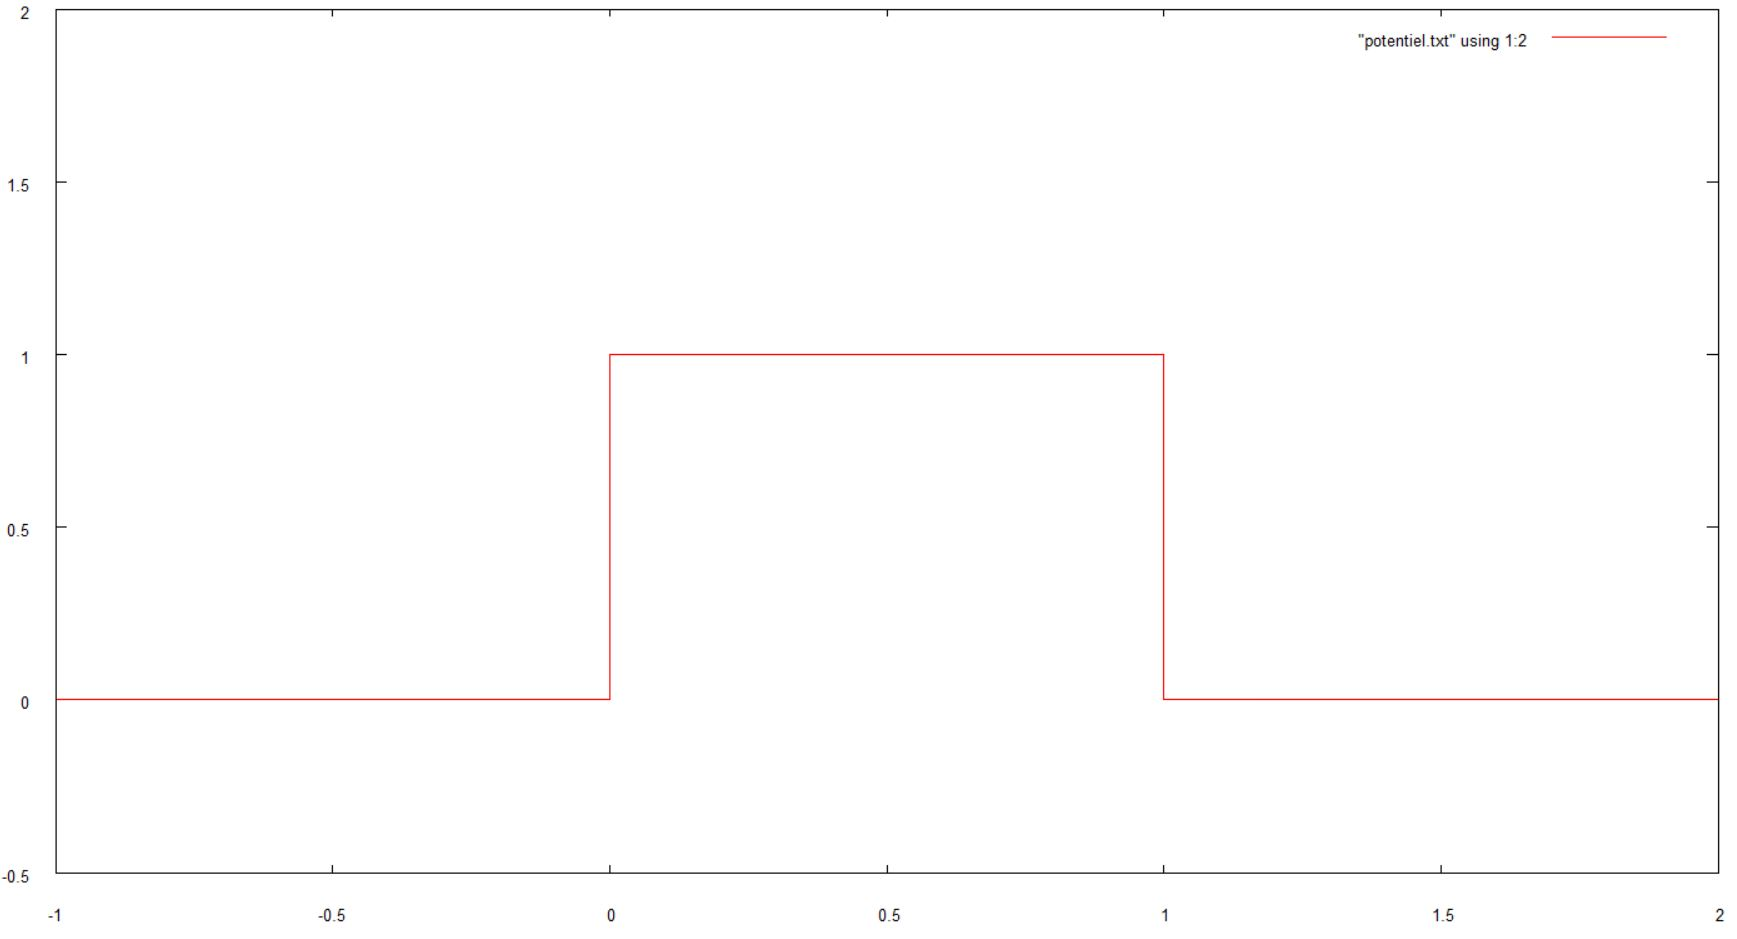
\includegraphics[width=0.4\textwidth]{potentielbarriere.jpg}
    \caption{Barrière de potentiel simple }
    \label{potentielbarriere}
\end{figure}

\begin{table}[!ht]
\centering
Paramètres utilisés  $a=1$,\ $m=1$,\ $V_{0}=1$,\ $N=20000$\\
\begin{tabular}{|l|l|l|}
\hline  Énergie & Coefficient de réflexion  & Coefficient de transmission \\
\hline  0.4 &   0.647581894537856 &  0.352418105437349\\
\hline 1 &  0.333366666342742 & 0.666633334211924\\ 
\hline 1.4 & 0.213549773737718 & 0.786450227124058\\
\hline
\end{tabular}
\caption{Coefficients de réflexion et transmission}
\label{tab3}
\end{table}

\subsection{ 2 Barrières de potentiels simples}

\begin{figure}[!ht]
    \center
    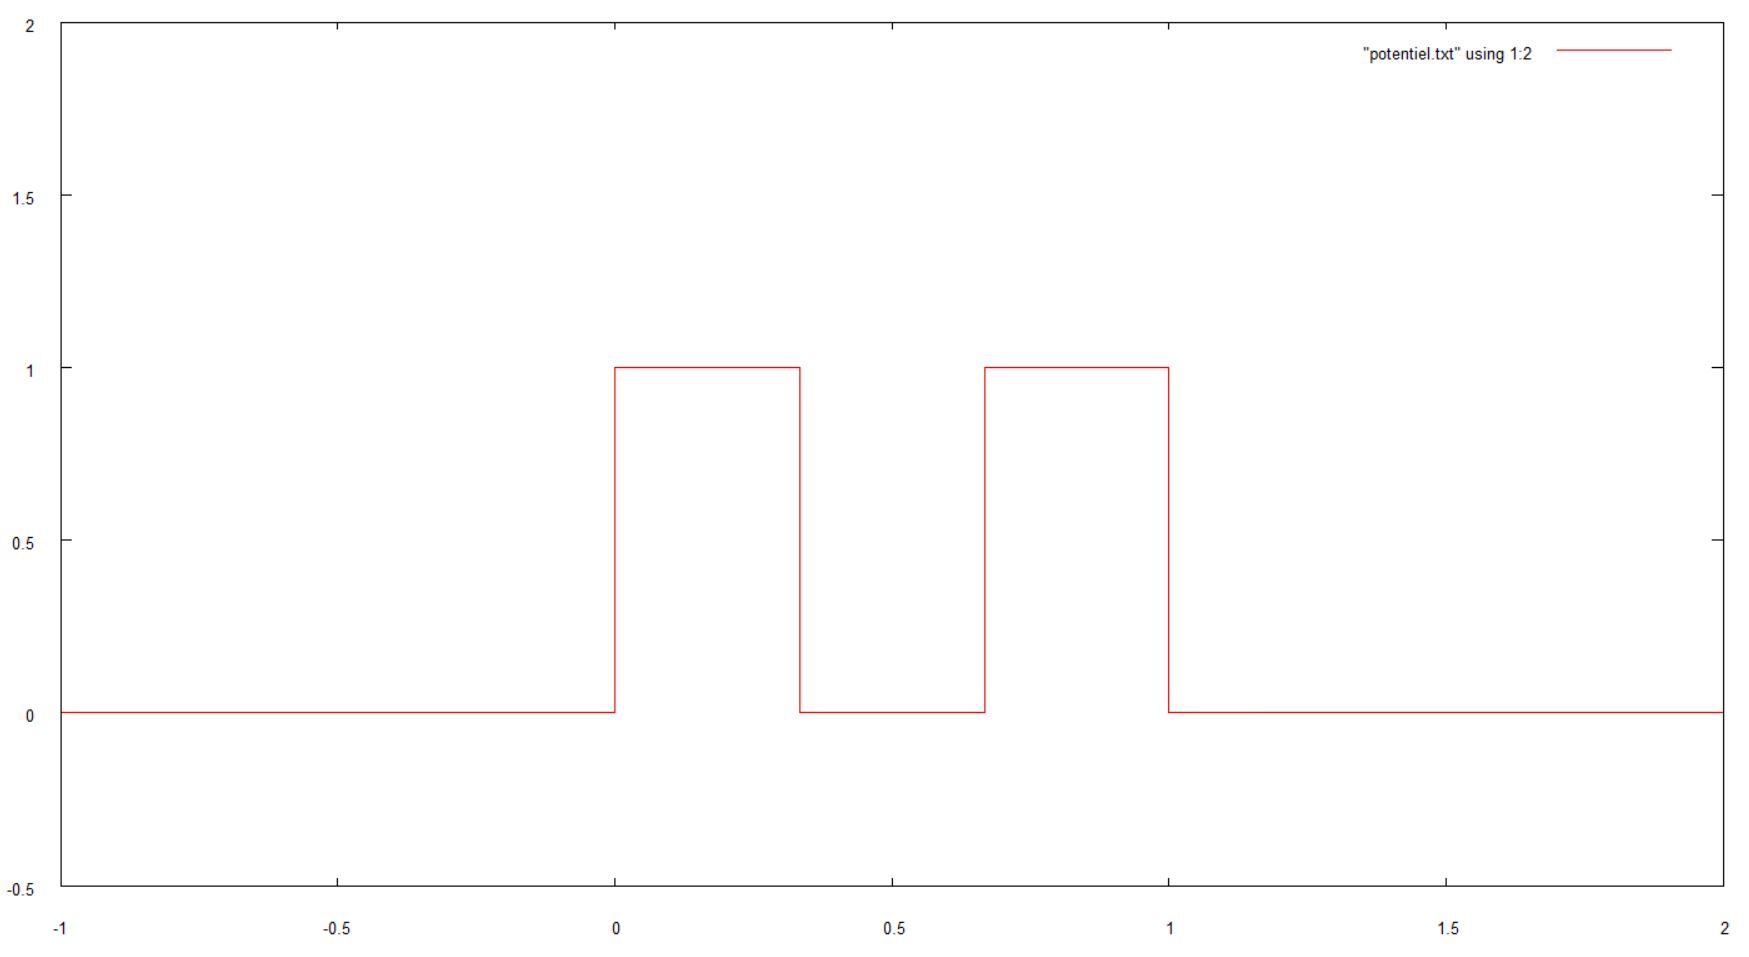
\includegraphics[width=0.4\textwidth]{potentiel2barriere.jpg}
    \caption{2 Barrières de potentiels simples }
    \label{potentiel2barriere}
\end{figure}

\begin{table}[!ht]
\centering
Paramètres utilisés  $a=1$,\ $m=1$,\ $V_{0}=1$,\ $N=20000$\\
\begin{tabular}{|l|l|l|}
\hline  Énergie & Coefficient de réflexion  & Coefficient de transmission \\
\hline  0.4 &  0.398212701243355 &  0.601787299006828\\
\hline 1 & 0.181835356681359 &0.818164643869745\\ 
\hline 1.4 & 0.123418941002287 & 0.876581059844542\\
\hline
\end{tabular}
\caption{Coefficients de réflexion et transmission}
\label{tab4}
\end{table}



\subsection{ 3 Barrières de potentiels simples}
\begin{center}

\end{center}
\begin{figure}[!ht]
    \center
    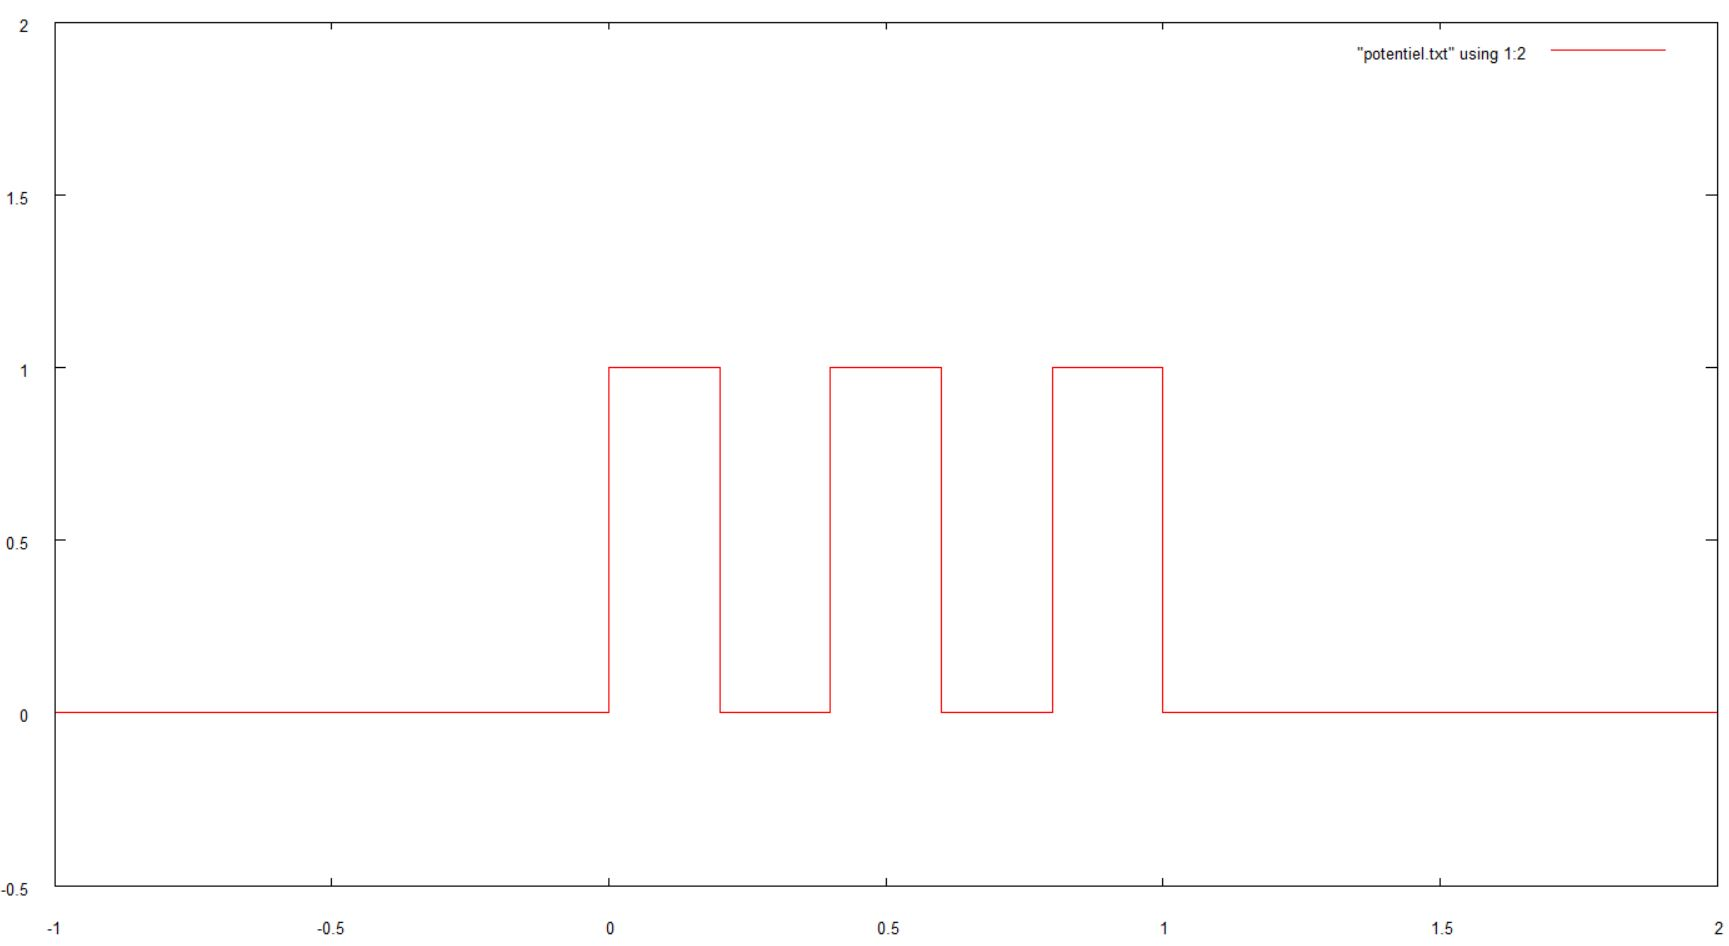
\includegraphics[width=0.4\textwidth]{potentiel3barriere.jpg}
    \caption{ 3 Barrières de potentiels simples}
    \label{potentiel3barriere}
\end{figure}

\begin{table}[!ht]
\centering
Paramètres utilisés  $a=1$,\ $m=1$,\ $V_{0}=1$,\ $N=20000$\\
\begin{tabular}{|l|l|l|}
\hline  Énergie & Coefficient de réflexion  & Coefficient de transmission \\
\hline  0.4 &   0.324948897997792 &  0.675051102149639\\
\hline 1 & 0.0951860743657358 & 0.904813926378733\\ 
\hline 1.4 &0.0456158378203416 & 0.954384163344269\\
\hline
\end{tabular}
\caption{Coefficients de réflexion et transmission}
\label{tab6}
\end{table}

\subsection{Barrière de potentiel gaussienne}
\begin{center}

\end{center}
\begin{figure}[!ht]
    \center
    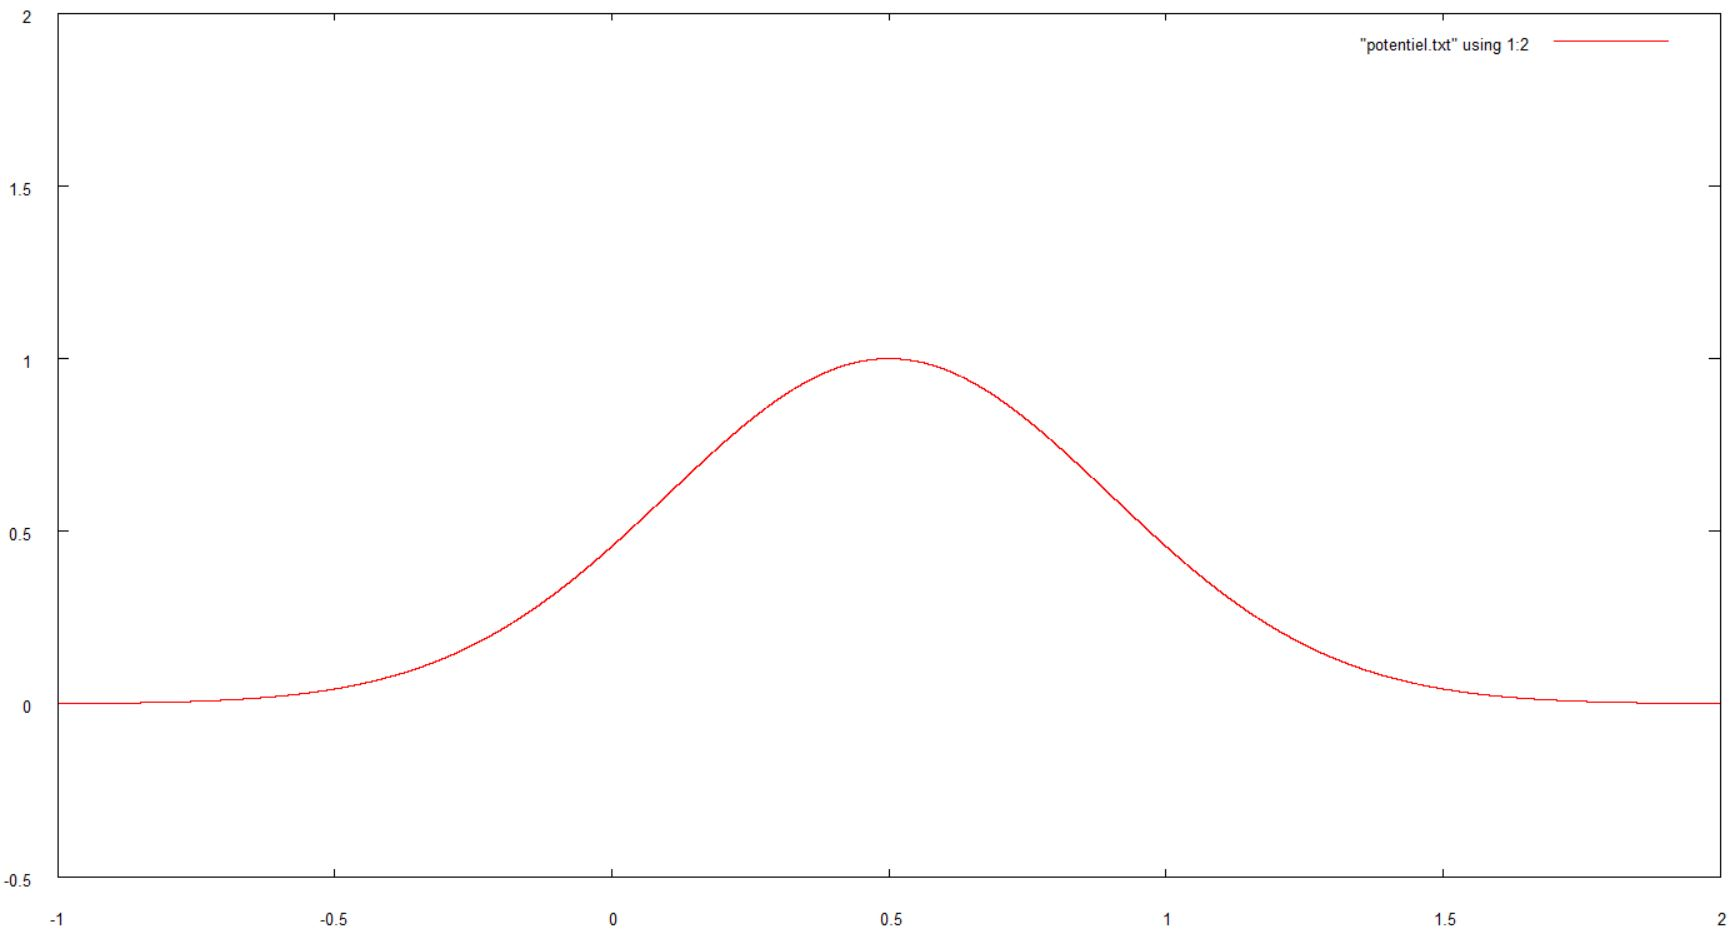
\includegraphics[width=0.4\textwidth]{barrieregaussienne.jpg}
    \caption{ Barrière de potentiel gaussienne}
    \label{barrieregaussiennne}
\end{figure}

\begin{table}[!ht]
\centering
Paramètres utilisés  $a=1$,\ $m=1$,\ $V_{0}=1$,\ $N=20000$\\
\begin{tabular}{|l|l|l|}
\hline  Énergie & Coefficient de réflexion  & Coefficient de transmission \\
\hline  0.4 &  0.0129595728676758 &  0.987040427735775\\
\hline 1 & 0.00462550868263464 & 0.995374492199424\\ 
\hline 1.4 & 0.0030585389705029 & 0.996941462224125\\
\hline
\end{tabular}
\caption{Coefficients de réflexion et transmission}
\label{tab7}
\end{table}

\subsection{Barrière de potentiel triangle}
\begin{center}

\end{center}
\begin{figure}[!ht]
    \center
    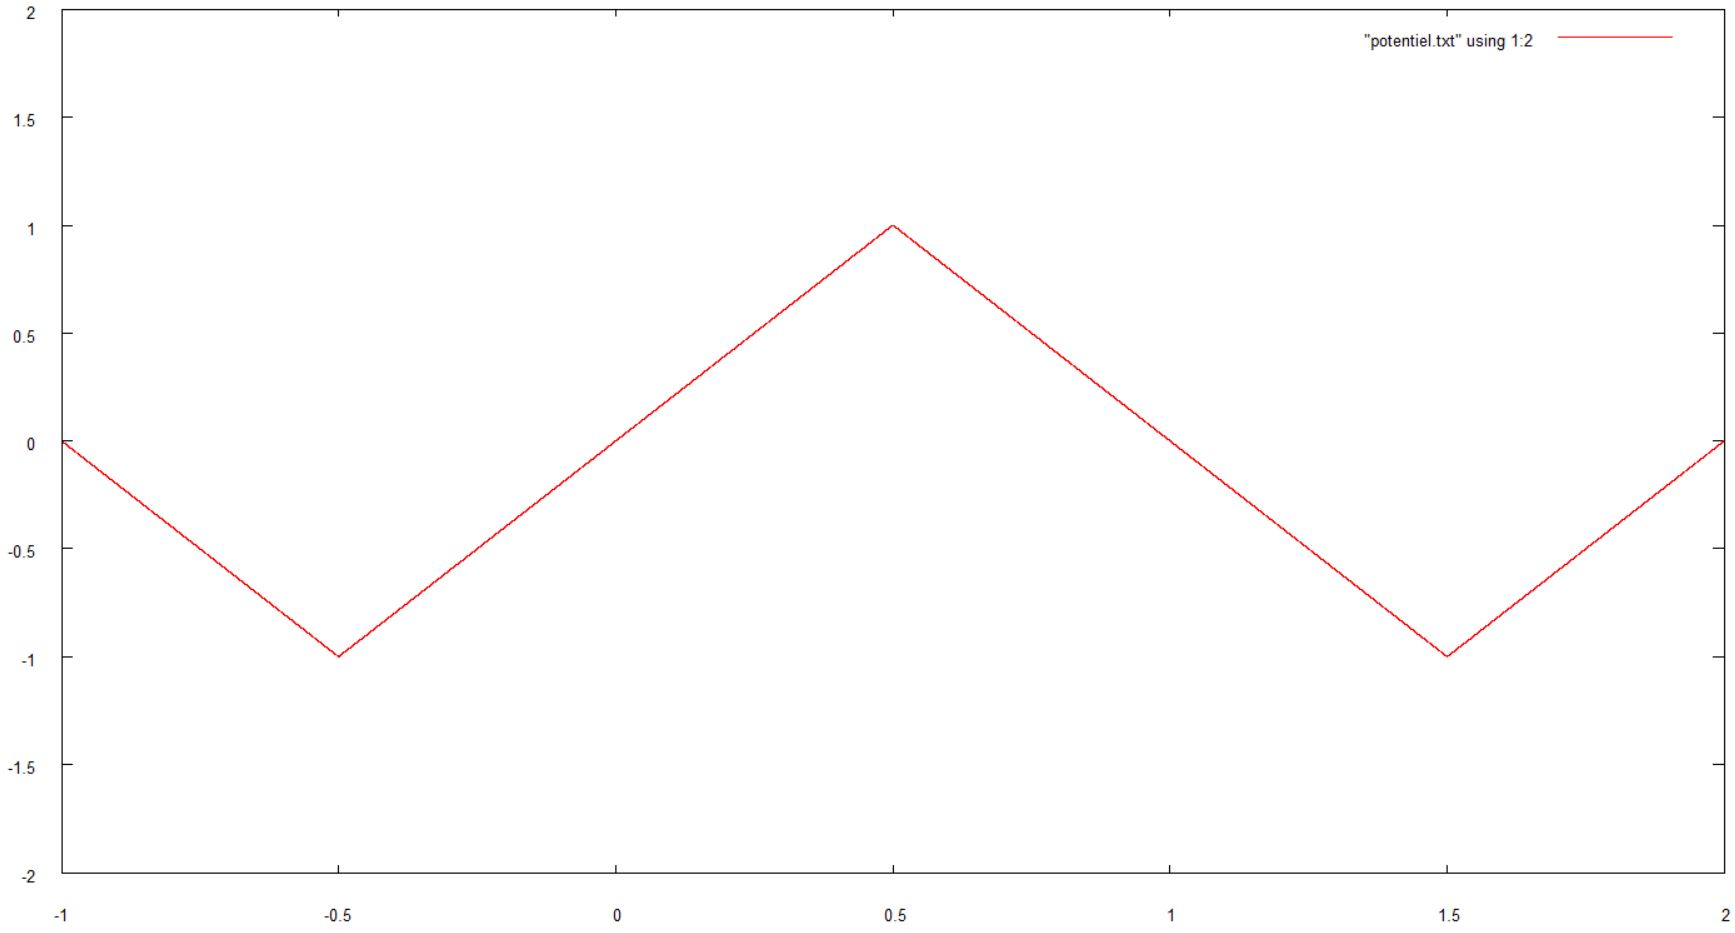
\includegraphics[width=0.4\textwidth]{potentieltriangle.jpg}
    \caption{ Barrière de potentiel triangle}
    \label{potentieltriangle}
\end{figure}

\begin{table}[!ht]
\centering
Paramètres utilisés  $a=1$,\ $m=1$,\ $V_{0}=1$,\ $N=20000$\\
\begin{tabular}{|l|l|l|}
\hline  Énergie & Coefficient de réflexion  & Coefficient de transmission \\
\hline  0.4 & 0.25435128942599 &  0.745648710947624\\
\hline 1 & 0.0947920470348868 & 0.905207953604588\\ 
\hline 1.4 &0.0588079770743296& 0.941192024180452\\
\hline
\end{tabular}
\caption{Coefficients de réflexion et transmission}
\label{tab}
\end{table}


Maintenant que nous avons déterminé les coefficients de transmissions et de réflexions pour les énergie de 0.4 ,1 ,1.4  Hartree.On peut voir que même avec des énergies inférieurs aux potentiels la transmission est non nul. On observe aussi que avec des énergies plus grandes que le potentiel la réflexion devient petite. Nous allons pour la suite nous intéresser à la variation des différents paramètres sur le coefficient de transmission.







  \cleardoublepage
  \section{Variation des paramètres}
\par Nous avons plusieurs paramètres a notre disposition pour définir la particule qui traversera le potentiel. Son état d'énergie initial et sa masse caractérise la particule. Nous pouvons choisir le type de potentiel pour simuler différent processus physique comme la désintégration Alpha que nous allons développer plus en dessous. 

\subsection{Variation de l’énergie}

\subsubsection{Particule Alpha}

 \par La radioactivité alpha est le rayonnement généré lors d'une \textit{désintégration alpha}, où un noyau atomique \textbf{X} éjecte une particule $\alpha$ composée de deux neutrons et de deux protons. Celle-ci se produit dans les atomes lourds tel que l'uranium 238, qui se transforme en thorium 234\cite{frwiki:200073754}. Dans le cadre de notre programme nous pouvons simuler la désintégration $\alpha$. Nous précisons le type de potentiel de type \textbf{Désintégration Alpha} pour générer la barrière de d'énergie qui retiendrait la particule par interaction nucléaire forte. Nous choisissons ensuite la largeur du potentiel comme 0.53 \si{\angstrom}, le rayon de Bohr comme la distance sur lequel l'effet tunnel va se réaliser. L'énergie au repos d'une particule $\alpha$ est de 3727.37 eV d'après le NIST\cite{enwiki:1148882523}. En Système d'unités atomiques celle-ci est de 137.8119 Hartree, qui nous convient comme entrée. Quand a la masse, nous entrons 4.00151 u\cite{NIST1}. Nous obtenons la courbe suivante pour la partie réel de la fonction d'onde $\Psi$.

 \begin{figure}[!ht]
     \centering
     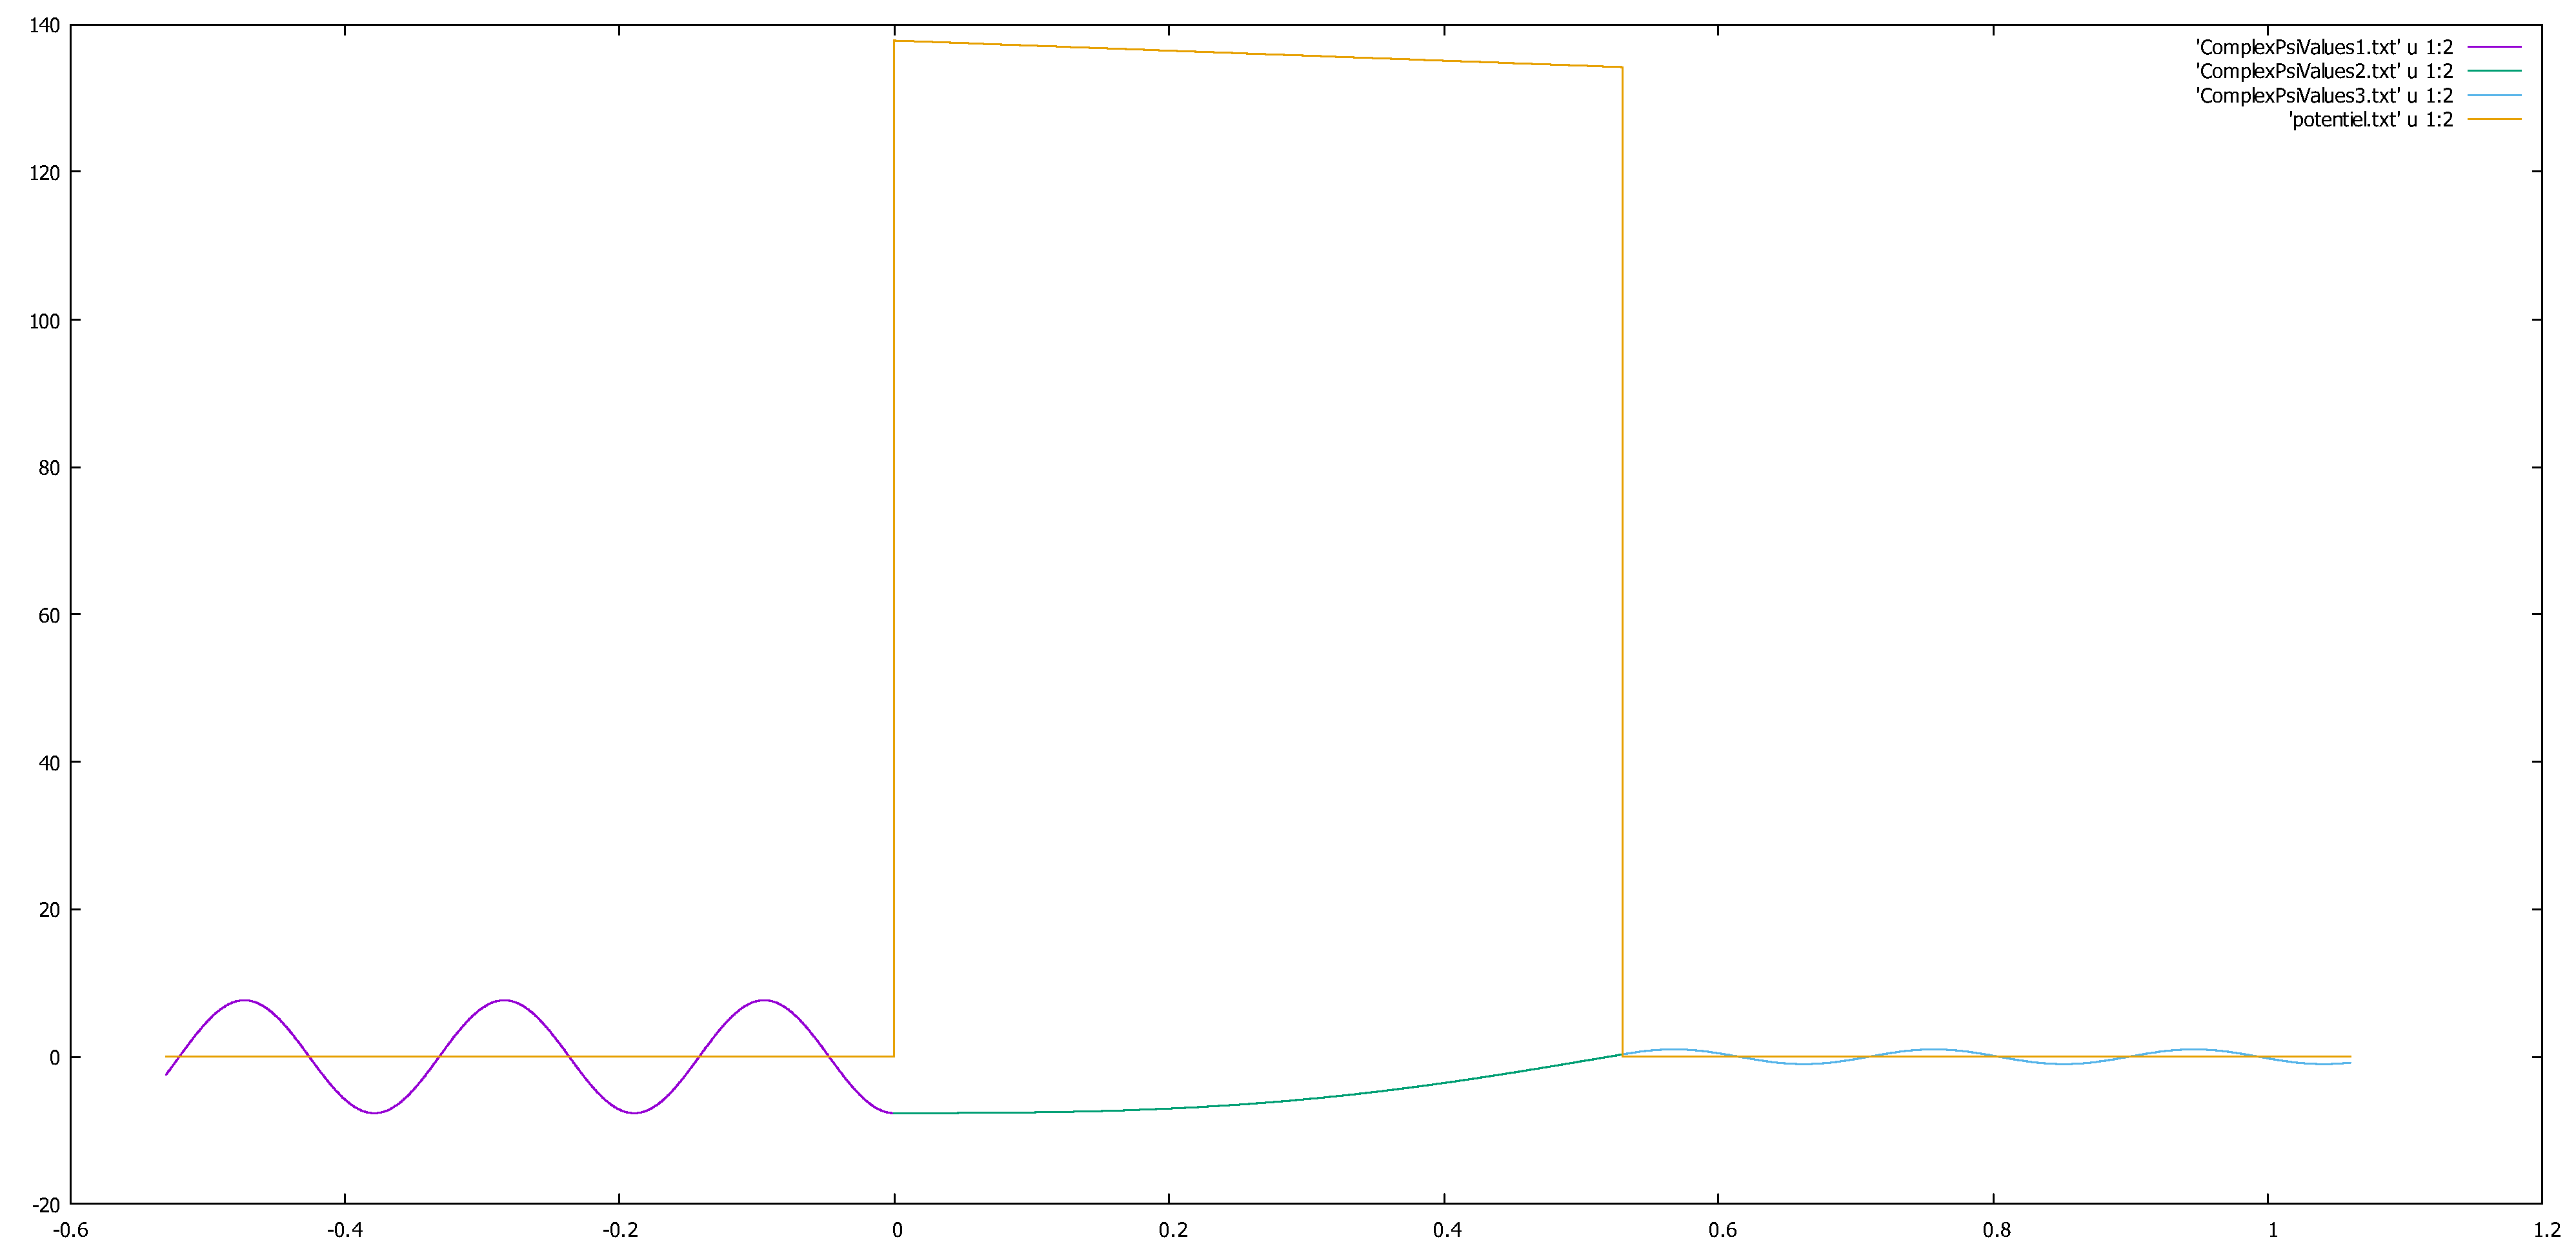
\includegraphics[width=0.4\textwidth]{Alpha/AlphaParticleDesintegration.pdf}
     \caption{Résolution Numérique de l'équation de Schrödinger pour une désintégration alpha}
     \label{fig:my_label}
 \end{figure}

\par En violet nous avons la courbe de l'onde en amont du potentiel et en bleu en aval de celle-ci.Nous observons le passage du fonction d'onde a travers le barrière en vert. Le coefficient de transmission pour cette application est calculé a T= 0.0632, d'où sur une grand nombre de phénomène de fission des particules traverse la barrière et sont émises. Le coefficient de réflexion quand a elle est de R= 0.9367.

\par Regardons a présent la courbe de Transmission en fonction de l'énergie du particule. 
\begin{figure}[!ht]
    \centering
    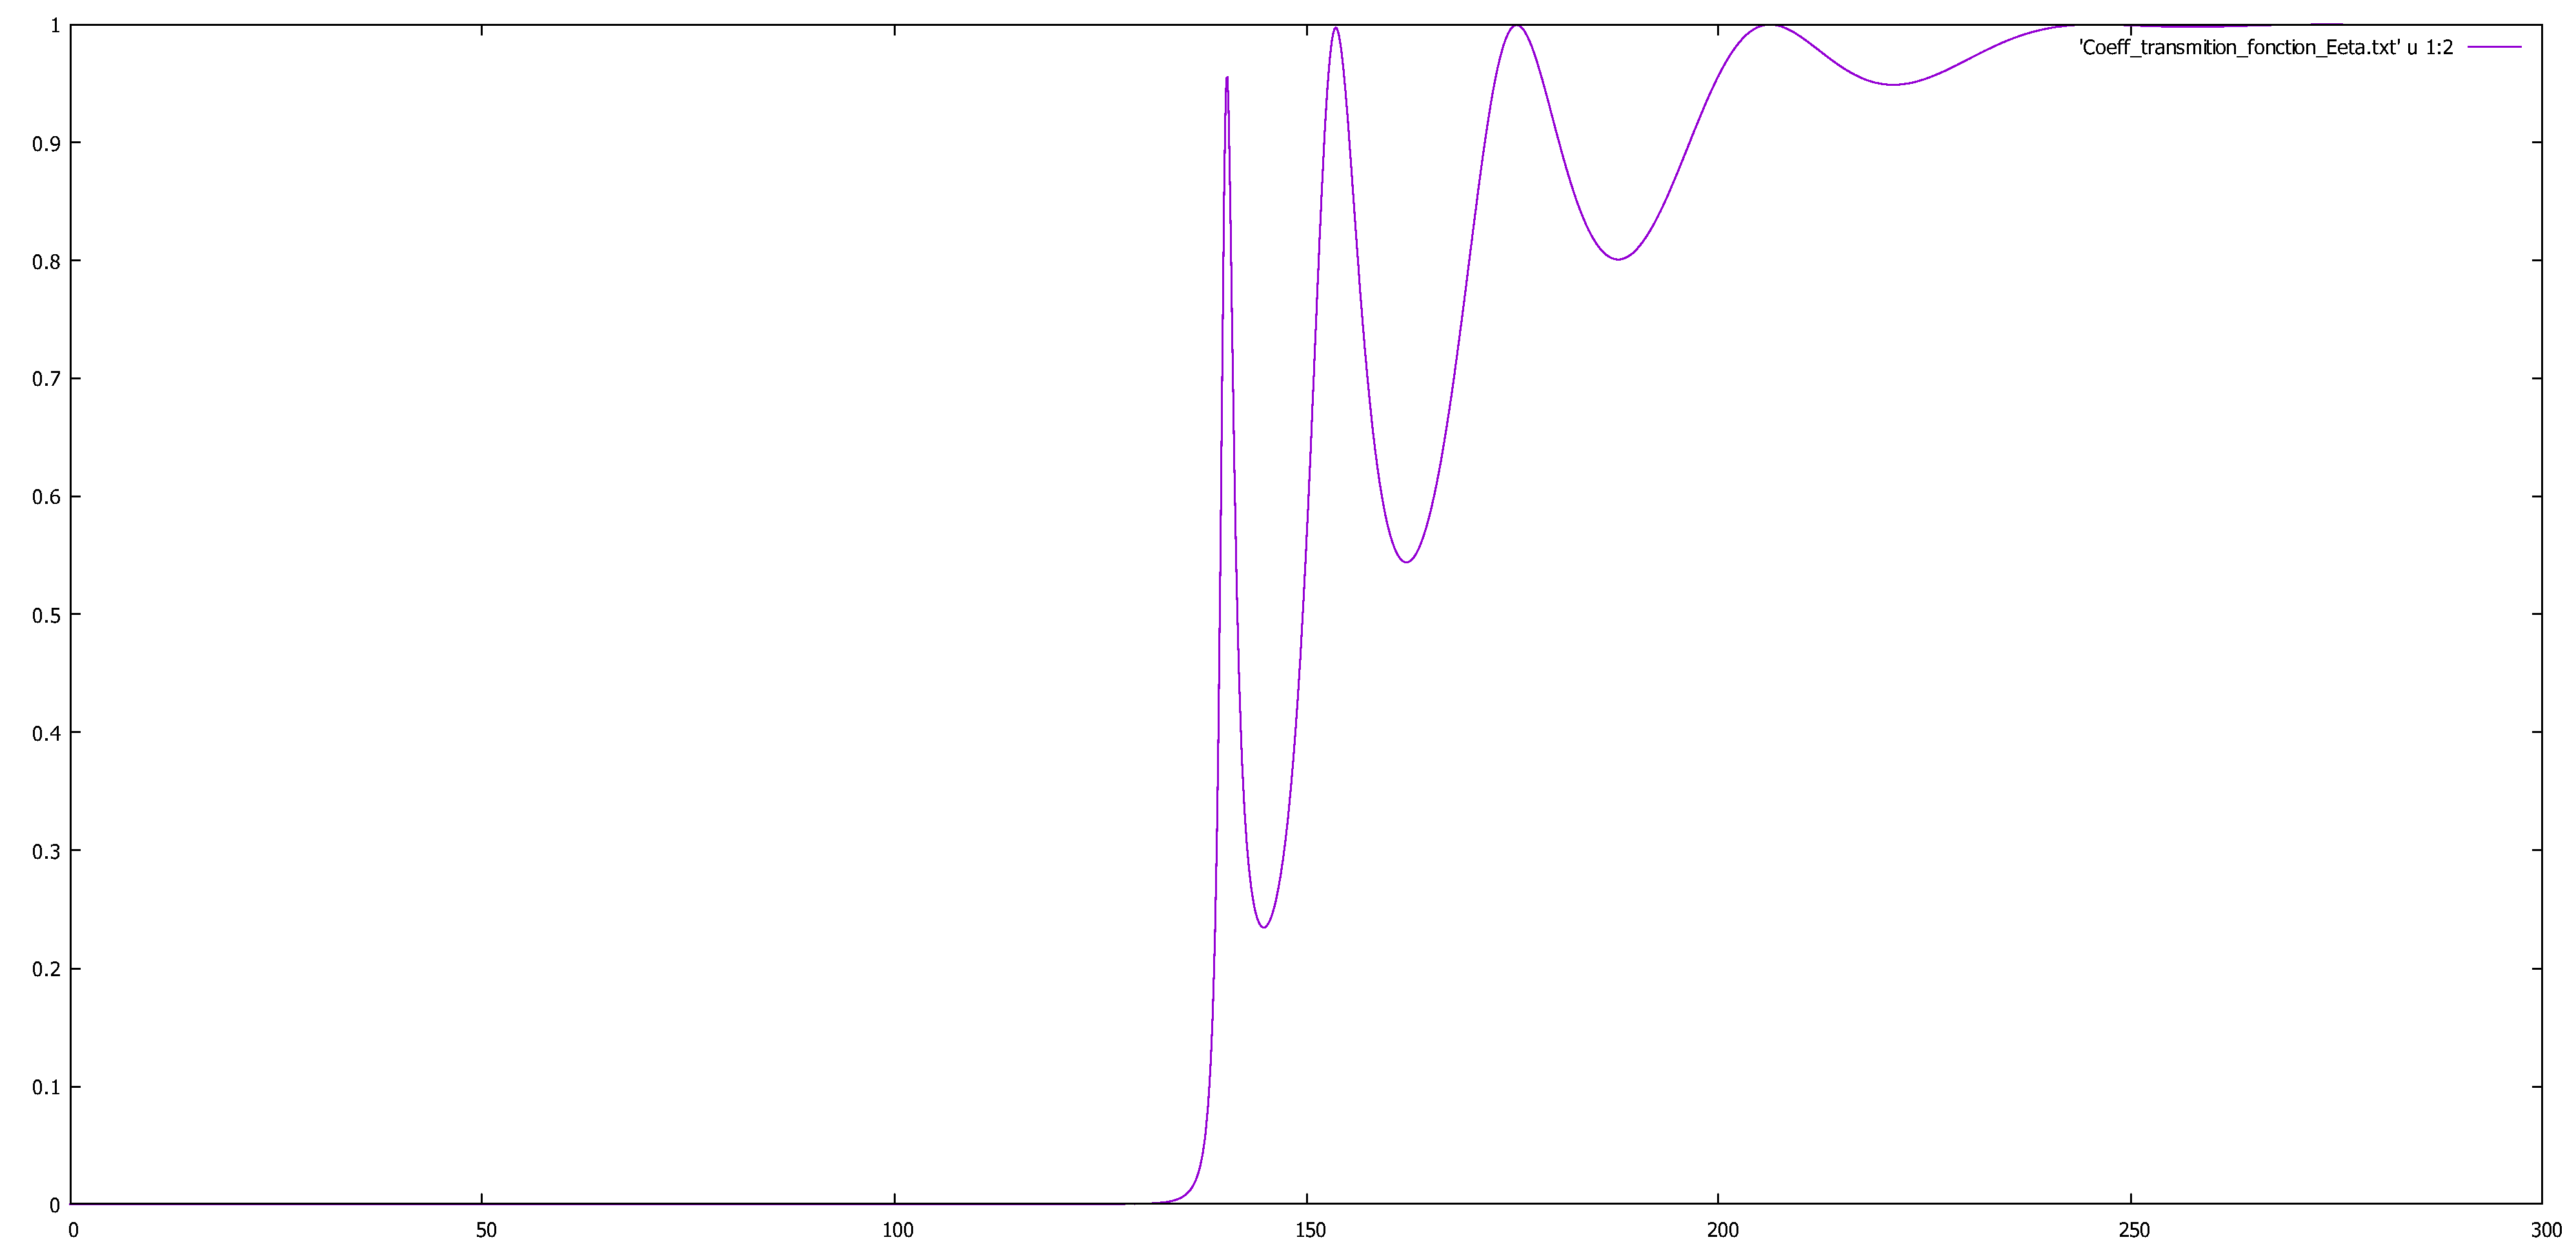
\includegraphics[width=0.4\textwidth]{Alpha/T(E).pdf}
    \caption{Coefficient de Transmission en fonction de l'énergie du particule alpha}
    \label{fig:my_label}
\end{figure}

Nous pouvons voir sur la fig.9, plusieurs valeur d'énergie pour lesquelles le coefficient de transmission est égale a 1 ou proche de 1. Pour observer ce qui se passe au niveau du premier pic, admettons les paramètres suivants:
\begin{table}[!ht]
\centering
Paramètres utilisés  $a=0.53$,\ $m=4.00151$,\ $V_{0}=140.56$,\ $N=10000$\\
\begin{tabular}{|l|l|l|}
\hline  Énergie & Coefficient de réflexion  & Coefficient de transmission \\
\hline  143.286 &  0.0787656025993423 &  0.921234397400658\\
\hline
\end{tabular}
\caption{Coefficients de réflexion et transmission}
\label{tab11}
\end{table}

\begin{figure}[!ht]
    \centering
    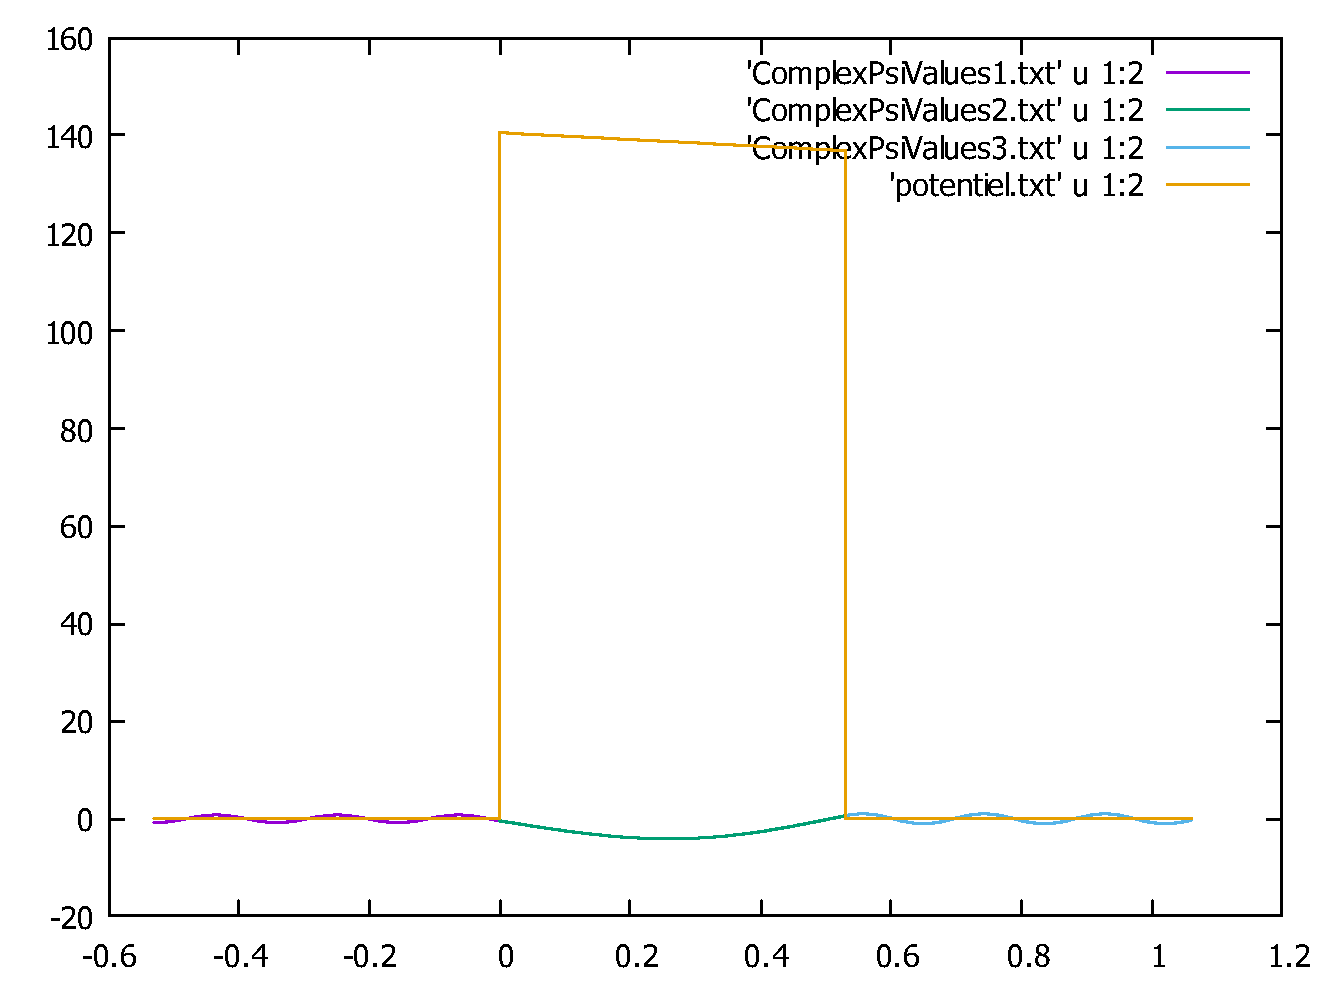
\includegraphics[width=0.6\textwidth]{AlphaResonnance/PsiReelResAplhaDecay.pdf}
    \caption{Capture du particule}
    \label{fig:my_label}
\end{figure}
\par Nous observons une particule en résonance avec le potentiel sur la figure 10. 

\subsubsection{Effet tunnel résonant}
\par L'effet tunnel est la capacité d'une particule quantique d'énergie inférieure a une seuil de franchir ce seuil. L'effet tunnel résonnant\cite{frwiki:182320873} quand a elle, apparaît lorsqu'une particule quantique aborde une tel système avec une énergie proche ou égale a celle du seuil. La probabilité de passage a travers les barrières est faible, mais la résonance avec le niveau des puits va piéger la particule, pendant une durée assez long, a l'intérieur du puits. Le coefficient de transmission de la particule est proche ou égale a l'unité dans ces instances. C'est pour cela que nous chercherons les résonances en observant la courbe de transmittivité en fonction de l'énergie lors de nos applications. 

\subsubsection{Capture de particule a travers une série de puits de potentiel}

\begin{table}[!ht]
\centering
Paramètres utilisés  $a=5$,\ $m=1$,\ $V_{0}=1$,\ $ N=20000 $\\
\begin{tabular}{|l|l|l|}
\hline  Énergie & Coefficient de réflexion  & Coefficient de transmission \\
\hline  0.47571 &  0.0202525776575487 &  0.979747422342451\\
\hline
\end{tabular}
\caption{Coefficients de réflexion et transmission pour une potentiel a 2 barrières}
\label{tab12}
\end{table}

\begin{figure}[!ht]
    \centering
    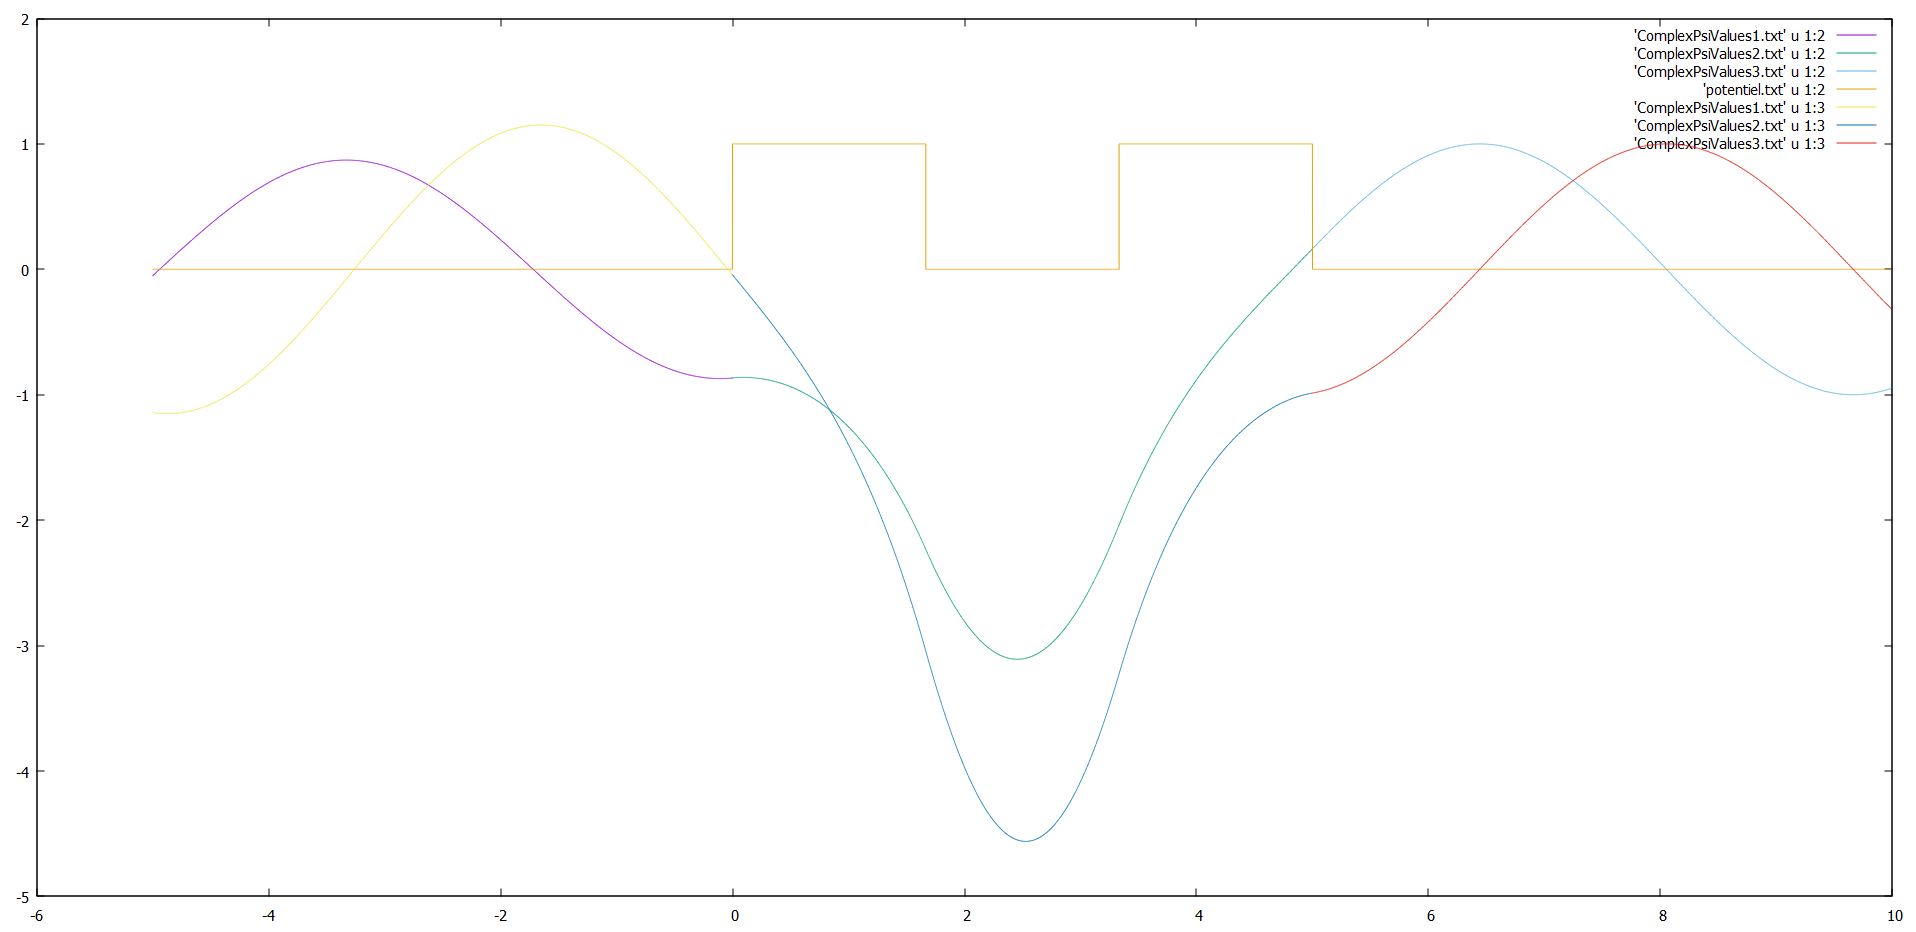
\includegraphics[width=0.8\textwidth]{2barriers Potentiel/2barReson.png}
    \caption{Capture du particule par 2 barrières de potentiel}
    \label{fig:my_label}
\end{figure}


\begin{table}[!ht]
\centering
Paramètres utilisés  $a=5$,\ $m=1$,\ $V_{0}=1$,\ $ N=20000 $\\
\begin{tabular}{|l|l|l|}
\hline  Énergie & Coefficient de réflexion 2 & Coefficient de transmission \\
\hline  0.606 &  0.0391264387378277 &  0.960873561262172\\
\hline
\end{tabular}
\caption{Coefficients de réflexion et transmission pour une potentiel a 3 barrières}
\label{tab12}
\end{table}

\begin{figure}[!ht]
    \centering
    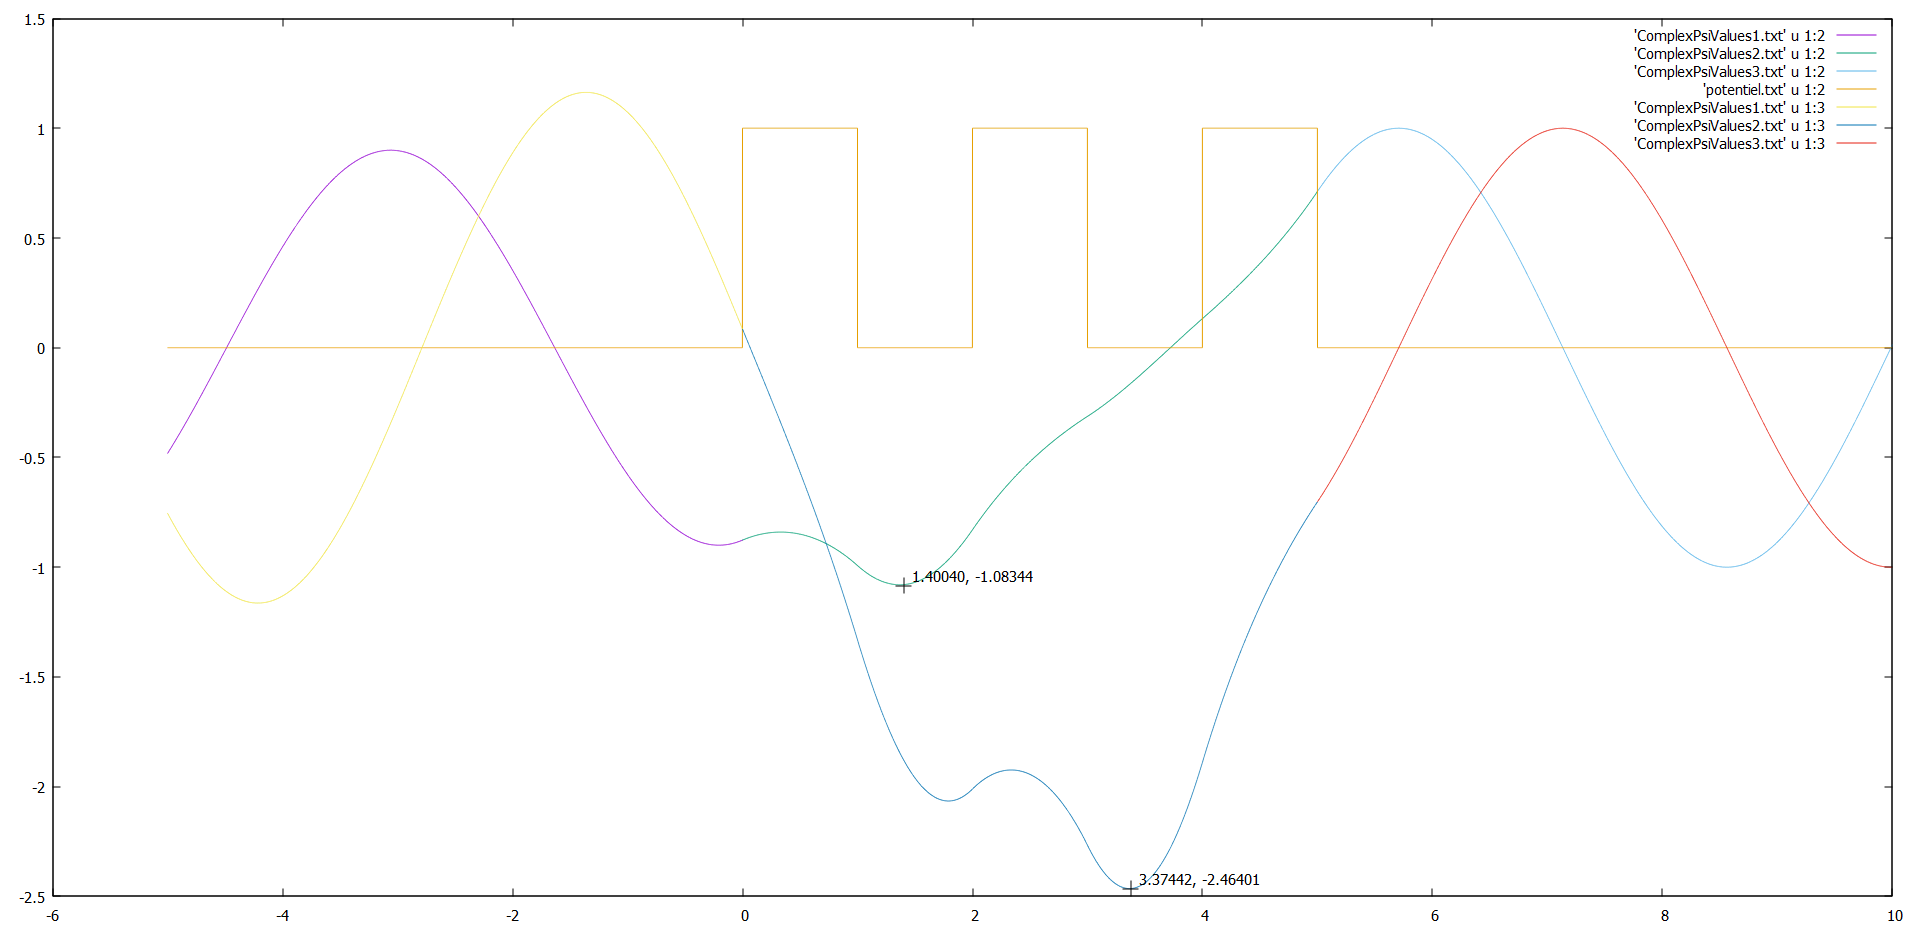
\includegraphics[width=0.8\textwidth]{3barriersResonnance/PsiReeletImaginaireReson.png}
    \caption{Capture du particule par 3 barrières de potentiel}
    \label{fig:my_label}
\end{figure}

\par Nous nous sommes positionné a la valeur de l'énergie de résonance, pour une série de puits de potentiel. 
\par Pour la fig. 11, nous remarquons que les parties réel et imaginaire de la fonction d'onde sont maximale et plus grand que le potentiel. La particule est bien capturée dans le puits démarqué par les deux barrières. 
\newpage
\par Pour la fig. 12, nous remarquons que la partie réel de la fonction d'onde est maximal est a l'unité au milieu du premier puits et que la partie imaginaire est maximal et plus grand que l'unité au niveau du second puits. En tenant en compte que le carré du fonction d'onde nous donne la densité de probabilité de présence du particule, nous pouvons en conclure que la particule est piégé au niveau du premier puits pour la plupart des réalisations de cette expérience.

\subsection{Variation de la taille du potentiel}

La variation du coefficient de transmission en fonction de la longueur du potentiel pour des énergies inférieurs à $V_{0}$. Pour une barrière de potentiel simple le coefficient de transmission sera décrit par la formule analytique \ref{eq:analityquee<v}. Si la condition $\alpha a >>1$ est vérifier le $sinh(\alpha a)$ va tendre vers $\frac{exp(\alpha a)}{2}$. Le coefficient de transmission va donc décroître exponentiellement.

\begin{center}
$T=\frac{16E(V_{0}-E)}{V_{0}^{2}}e^{-2\alpha a}$\\
paramètres utilisés $E=0.1$,\ $m=1$,\ $V_{0}=1$
\end{center}
\begin{figure}[!ht]
    \center
    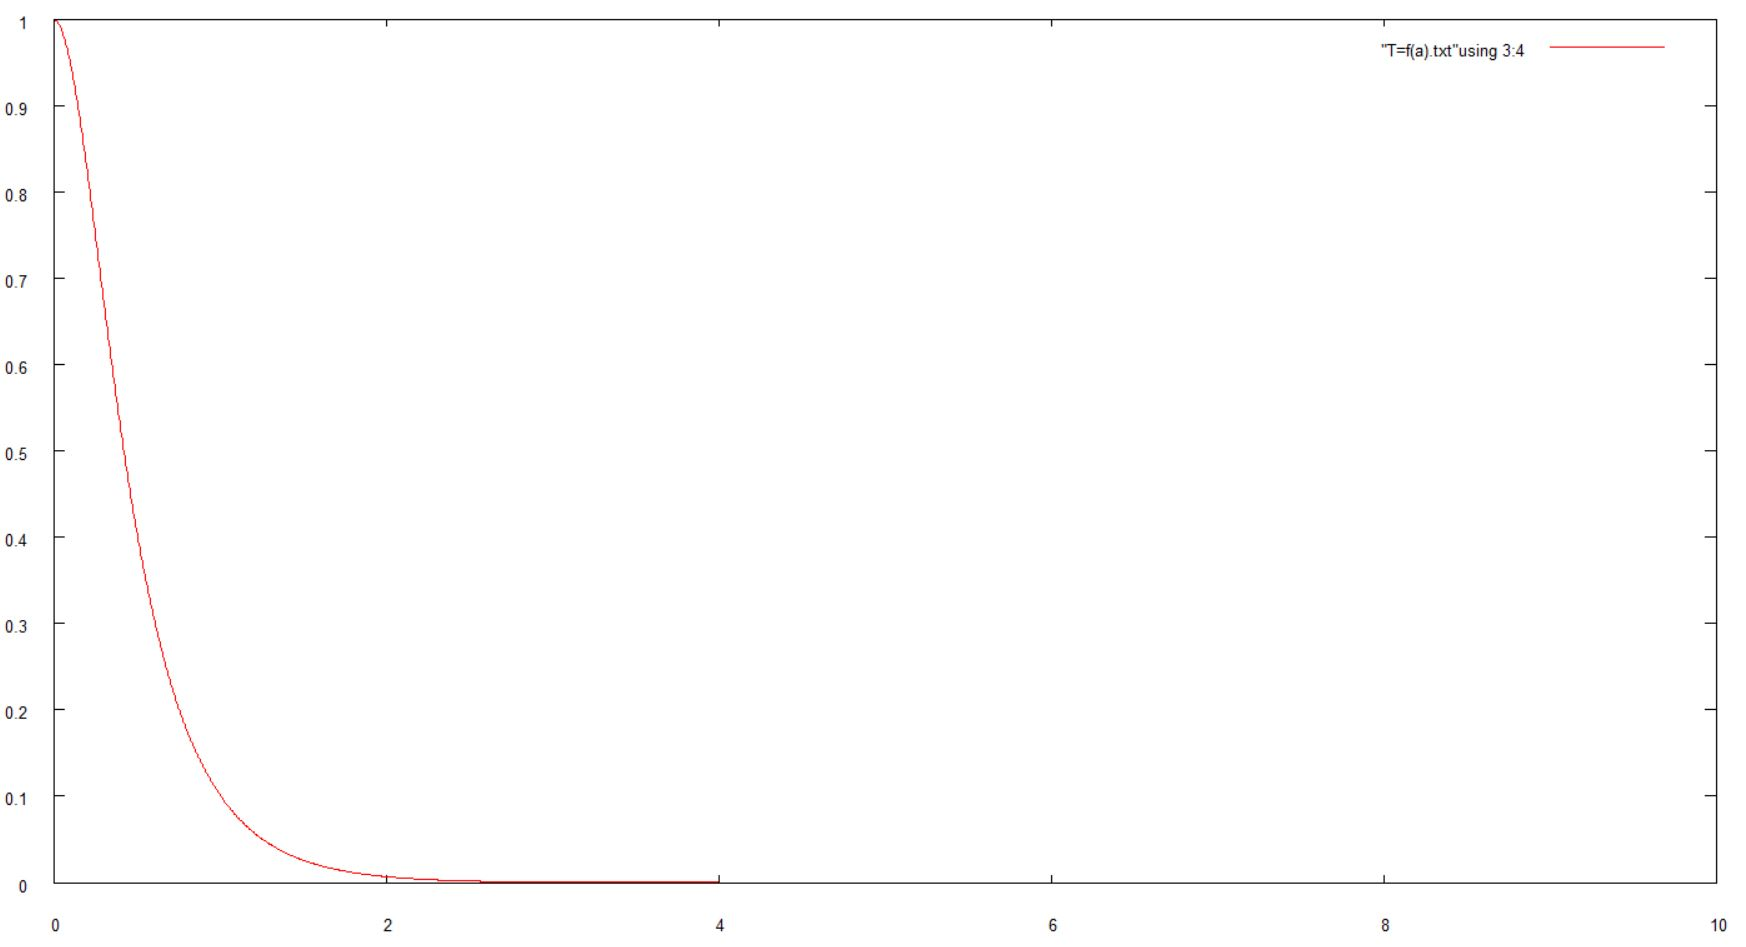
\includegraphics[width=0.5\textwidth]{t=f(a).jpg}
    \caption{Coefficient de transmission en fonction de x }
    \label{t=f(a)}
\end{figure}

Cette propriété de décroissance du coefficient de transmission est exploité par le microscope à effet tunnel. Le principe du STM  (scanningtunneling microscope) est d'approcher une pointe de la surface que l'on veut cartographier, la distance entre la pointe et la surface peut être assimiler à une barrière de potentiel. Lorsque l'on est suffisamment  proche on détecte un courant qui est transmit par effet tunnel. Le courant va suivre la même décroissance que le coefficient de transmission se qui permet d'avoir des résolutions de la surface inférieur à la taille d'un atome.



\subsection{Variation de la masse}

\begin{figure}[!ht]
    \centering
    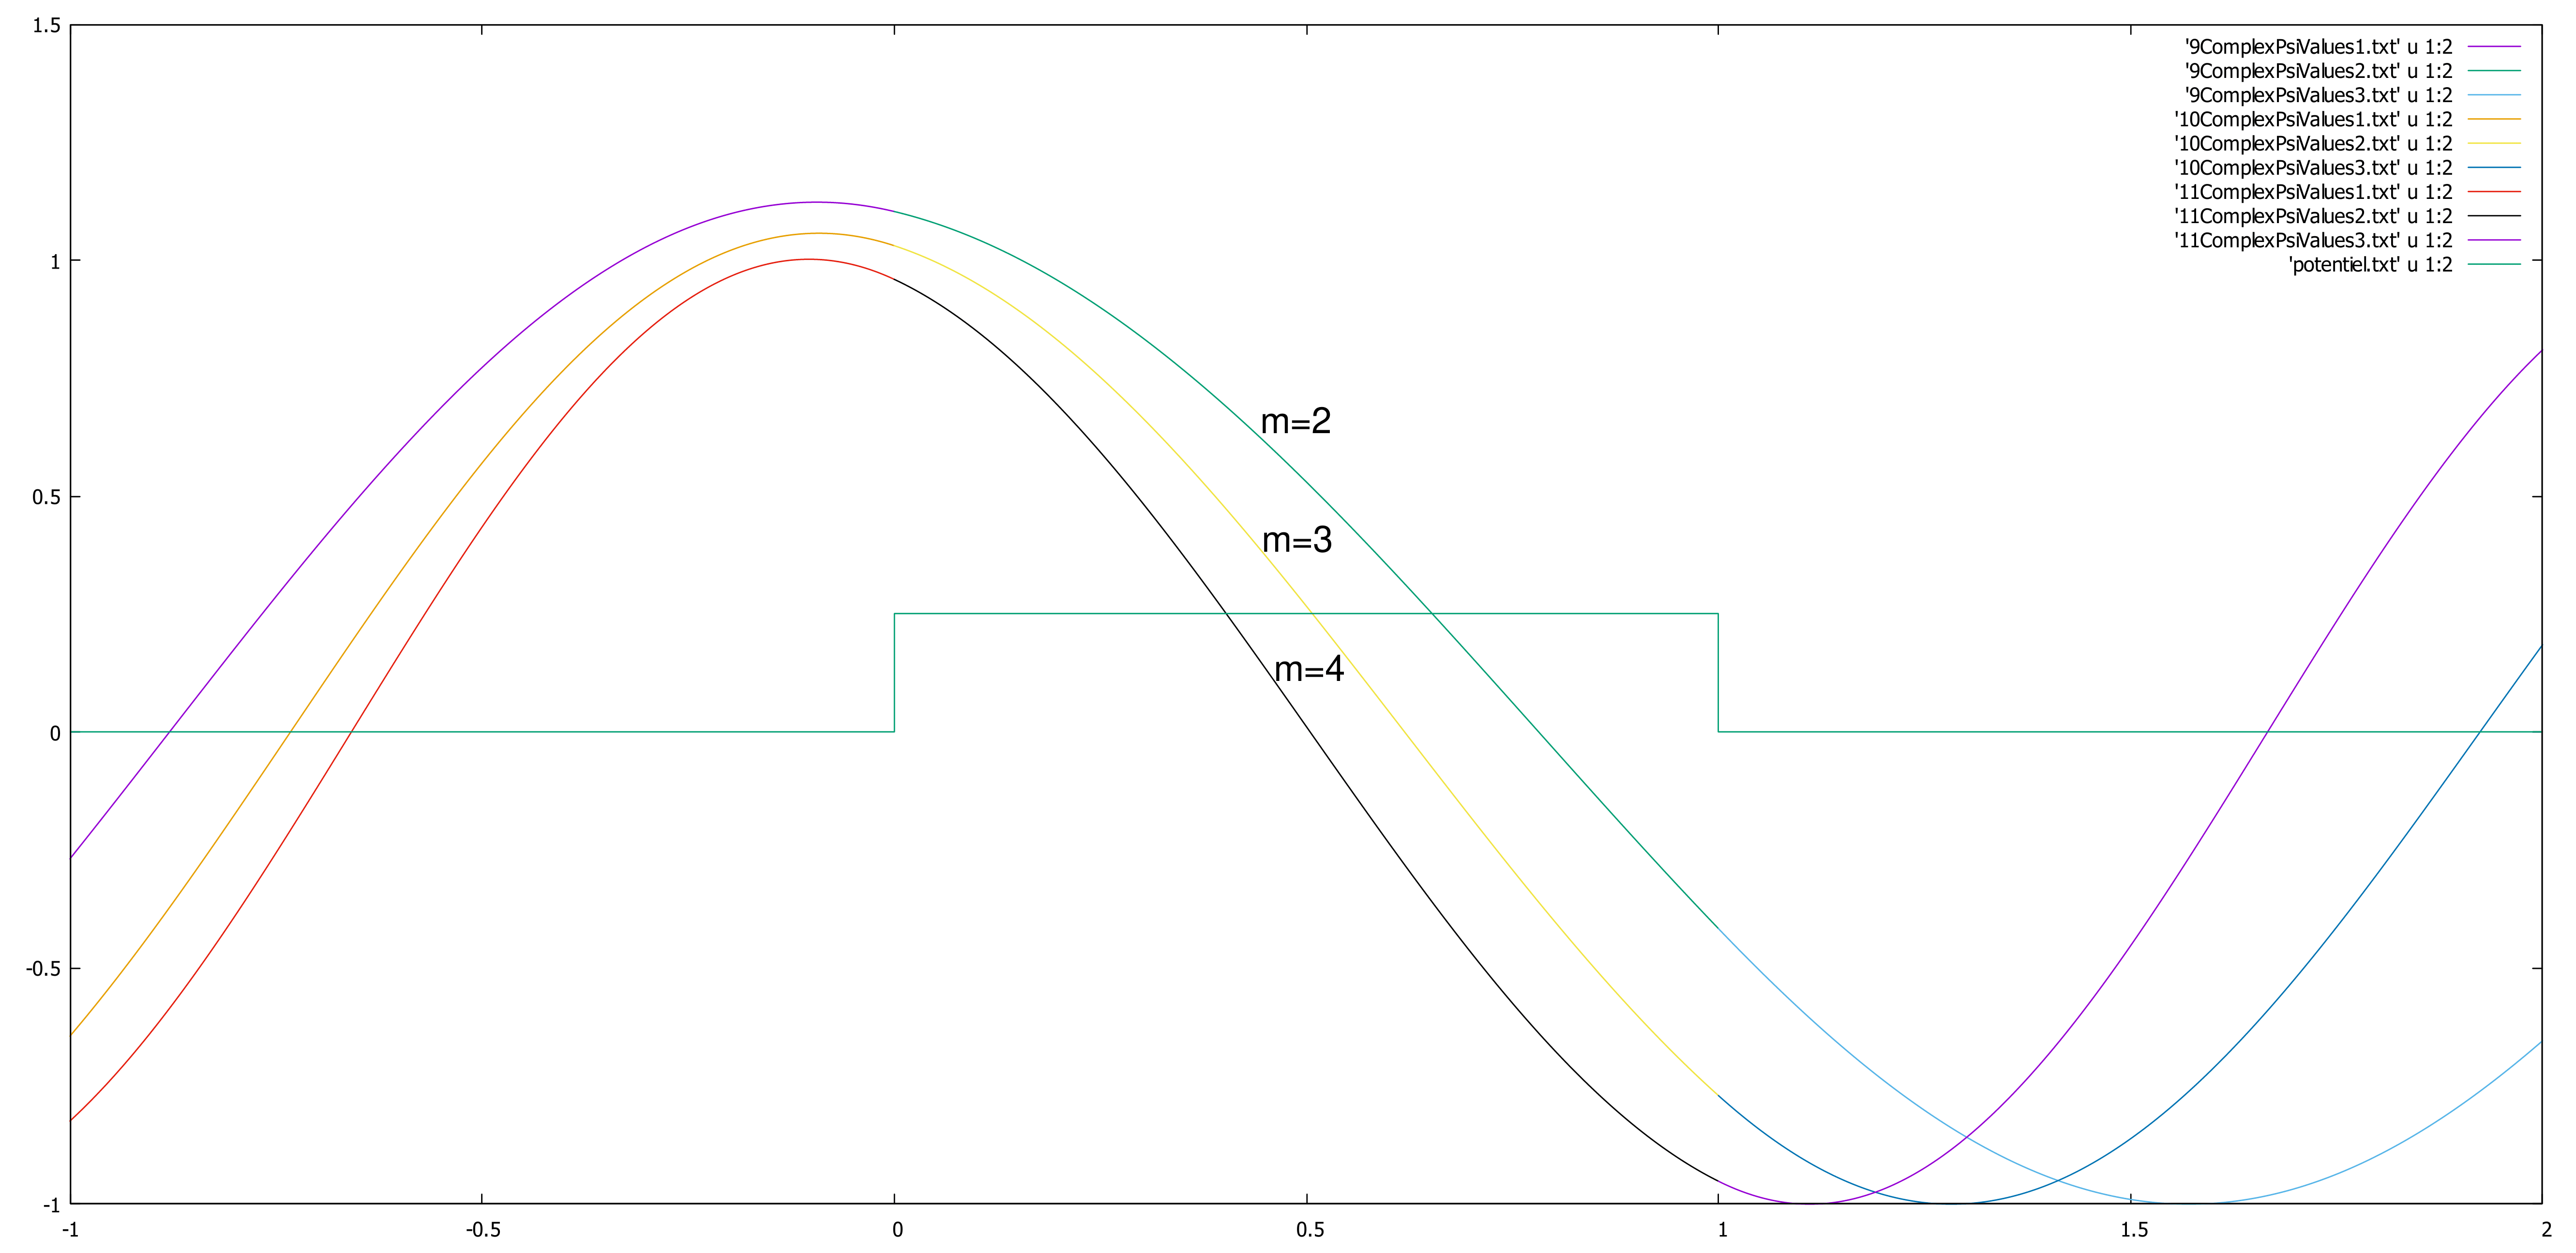
\includegraphics[width=0.8\textwidth]{potentiel 1 barrier/m augmentant seul2-1.png}
    \caption{Partie réel de $\Psi$(x) avec m comme paramètre fluctuant}
    \label{fig:my_label}
\end{figure}

\begin{table}[!ht]
\centering
Paramètres utilisés $E=1$,\ $a=1$,\ $V_{0}=0.25$,\ $N=20000$\\
\begin{tabular}{|l|l|l|}
\hline  masse & Coefficient de réflexion  & Coefficient de transmission \\
\hline  2 & 0.0198908911855625 &  0.9801091104902894\\
\hline 3 & 0.014900596680466 & 0.985099405784575\\ 
\hline 4 & 0.00840550290054031&0.991594500394001\\
\hline
\end{tabular}
\caption{Coefficients de réflexion et transmission}
\label{tab}
\end{table}
  \cleardoublepage
  \section*{Conclusion}
\addcontentsline{toc}{section}{Conclusion}

\par Pour conclure, nous avons modélisé plusieurs types de barrières de potentiels et réalisé le calcul numérique de la fonction d'onde et ainsi trouver les coefficients de réflexion et de transmission pour différentes énergies et masses. Par l'usage de l'interface graphique GNUplot, nous avons réalisé les courbes de Re($\Psi$(x)) et observé la capture de particule avec le phénomène de résonance. Il nous à été possible de montrer que à certaine énergie il est possible d'obtenir la transparence du potentiel pour avoir un coefficient de transmission égale à 1. La visualisation de l'effet tunnel permet aussi de comprendre le fonctionnement du microscope à effet tunnel.
Enfin pour ce qui pourrait êtres intéressant pour d'autre développement du programme, la résolution de l'équation de Schrödinger à plusieurs dimensions.

  \cleardoublepage
 
  \bibliographystyle{plain}
    \bibliography{reference}
    

\end{document}

